\documentclass[12pt]{article}
\usepackage{setspace}
\doublespacing
\usepackage{listings}
\lstset{language=Python, showstringspaces=false}
\usepackage{tikz}
\usetikzlibrary{arrows,snakes,calc}
\tikzstyle{input}=[circle,draw=blue!50,fill=blue!20,thick,minimum size=10mm]
\tikzstyle{hidden}=[circle,draw=gray!50,fill=gray!20,thick,minimum size=10mm]
\tikzstyle{output}=[rectangle,draw=orange!50,fill=orange!20,thick,minimum size=10mm]
\tikzstyle{pre}=[<-]
\newcommand{\ystep}{-2.5}


\usepackage[a4paper, total={6.27in, 9.69in}]{geometry}
\usepackage[rightcaption]{sidecap}
\usepackage{graphicx}
\usepackage{wrapfig}
\usepackage{url}
\usepackage[titletoc,title]{appendix}
\usepackage{amsmath}
\usepackage{amssymb}

\newcommand{\R}{\mathbb{R}}
\newcommand{\rdim}[2]{\mathbb{R}^{#1 \times #2}}
\newcommand{\hyp}{h_\Theta(x)}
\newcommand{\D}{\frac{\partial}{\partial \Theta_{i,j}^{(l)}}J(\Theta)}

\graphicspath{ {../Images/} }

\begin{document}
\pagenumbering{roman}
\begin{titlepage}
  \thispagestyle{empty}
  \begin{center}
    \begin{singlespacing}
    \vspace*{1cm}

    
    \Huge
    \textbf{Exploring Teacher Forcing Techniques for Sequence-to-Sequence Abstractive Headline Summarization}

    
    \vspace{1.0cm}
    

    \vspace{3.5cm}

    \Large
    \textbf{Corbin Albert}
    

    \vfill

    \textbf{Supervisor: Dr. Natasa Milic-Frayling}\\
    \vspace{1.5cm}
    A dissertation presented for the degree of\\
    Masters of Computer Science and Artificial Intelligence

    
    \vspace{0.8cm}

    
    
\includegraphics[width=0.4\textwidth]{university}

    \Large
    Department of Computer Science\\
    University of Nottingham\\
    United Kingdom\\
    \today
  \end{singlespacing}
  \end{center}
\end{titlepage}
\clearpage

\begin{onehalfspacing}
\section*{Abstract}
Every internet user today is exposed to countless article headlines. These can range from informative, to sensationalist, to downright misleading. These snippets of information can have tremendous impacts on those exposed and can shape ones views on a subject before even reading the associated article. For these reasons and more, it is important that the Natural Language Processing community turn its attention towards this critical part of everyday life by improving current abstractive text summarization techniques. To aid in that endeavor, this project explores various methods of teacher forcing, a technique used during model training for sequence-to-sequence recurrent reural network architectures.

A relatively new deep learning library called PyTorch has made experimentation with teacher forcing accessible for the first time and is utilized for this purpose in the project. Additionally, to the author's best knowledge this is the first implementation of abstractive headline summarization in PyTorch. Seven different teacher forcing techniques were designed and experimented with: (1) Constant levels of  0\%, 25\%, 50\%, 75\%, and 100\% teacher forcing probability through the entire training cycle; and (2) two different graduated techniques: one that decreased linearly from 100\% to 0\% through the entire training cycle to convergence, and another that graduated from 100\% to 0\% every 12.5\% of the training cycle, often corresponding with learning rate annealing. Dozens of generative sequence-to-sequence models were trained with these various techniques to observe their differences.

These seven different teacher forcing techniques were compared to one another via two metrics: (1) ROUGE F-scores, the most common metric used in this field; and (2) average loss over time. Counter to what was expected, this project shows with statistical significance that consistent 100\% and 75\% teacher forcing produced better ROUGE scores than any other metric.

These results confirm the use of 100\% teacher forcing, the most widely used technique today. However, this throws into question an important assumption by many leading machine learning researchers that dynamic, graduated teacher forcing techniques should results in greater model performance. Questions of ROUGE metric validity, response to more complicated model parameters, and domain specificity are encouraged for further analysis.
\end{onehalfspacing}
\newpage
\section*{Acknowledgements}
There are too many people to name I have depended on throughout the completion of this MSc, but I shall try to name but a few.
\\
\\
First and foremost I must thank Alexandra Din, who showed such incredible love, support and selflessness throughout my postgrad.
\\
\\
To my parents, without whom I could never have had such a tremendous opportunity at personal growth.
\\
\\
To Soofi Din, for being the greatest friend and conversationalist I have ever known.  And to Amanda Din, for always pushing me to do my best and keeping me on my toes.
\\
\\
Quite especially to Jeremy Howard of fast.ai. Without his deep learning MOOC, I could never have gained the requisite knowledge to understand and build deep neural networks.
\\
\\
To my classmates turned friends at The University of Nottingham for sharing in your passion for this great field of Computer Science.
\\
\\
To The University of Pennsylvania's Linguistic Data Consortium for their generous scholarship for the Annotated English Gigaword Corpus so paramount to the implementation and success of this project.
\\
\\
To my Supervisor, Dr. Natasa Milic-Frayling, for her much appreciated guidance and encouragement.
\\
\\
And to all the faculty of The University of Nottingham whom had the great misfortune have having to put up with me.

\newpage
\tableofcontents
\newpage
\listoffigures
\newpage
\listoftables
\newpage
\pagenumbering{arabic}

\section{Introduction}\label{intro}

Article headlines play an increasingly important role in today's information-dense world. Their intent is to be a highly digestible summary of the information contained within the associated article so the reader can decide whether the content will be of interest. But they also need to hook the reader in and grab their attention. In the days of newspaper media, this may have only applied to front-page headlines, enticing a potential reader to buy the paper. In the age of online journalism, however, every article is an opportunity to generate revenue by having readers visit their site. Setting aside the 24-hour news cycle from any one particular publication, resources like Reddit, Twitter and Facebook enable and indeed profit from their users seeing dozens if not hundreds of headlines every day.

This becomes a problem when people start are so inundated with information that they propagate headlines uninformed of the contents within. Take, for instance, a recent report that uncovered that 59\% of articles on Twitter were never clicked or read before being shared~\cite{Gabielkov2016}. Even for issues that an individual deems important, the headline is often the only exposure to the information that said person has had. Headlines can also cause substantive misconceptions for those who do not read the article as well~\cite{Wenzlaff1981}.

Furthermore, in the case of misleading headlines, evidence has shown that, even for individuals that read the associated articles, biases are created from the first impressions that headlines form~\cite{Ecker2014}. Even if the misleading element(s) of the headline is addressed within the article, the reader is still more likely to be misinformed after fully reading the article content~\cite{Ecker2014}. The first impressions that headlines provide are nearly impossible to overcome. It truly is difficult to overstate their importance.

Suffice it to say, headlines play a crucial role in our daily digestion of information and deserve the attention of the Natural Language Processing (NLP) community. Unfortunately, we are still many years away from being able to tackle some of the more pressing concerns revolving around headlines and their effect on the public. We are currently still in the early stages of generating headlines from article content, but this means that there are many interesting questions to explore.

Therefore, this research project hopes to contribute to the field of abstractive text summarization (Sec.~\ref{textsum}) by exploring one of the open questions. Current undertakings within this area of interest have used attentional sequence-to-sequence models (seq2seq; Sec.~ref{seq2seq}), a type of Recurrent Neural Network (RNN; Sec.~\ref{rnn}) to achieve the best results thus far. But teacher forcing (Sec.~\ref{tf}), a method used to help train seq2seq models, has not been explored in great depth, nor have the capabilities been realized until recently. Therefore, this project focuses on studying the effects of various teacher forcing techniques for the task of headline summarization, in an attempt to help guide the direction of future seq2seq research.
\section{Literature Review}\label{litrev}

\subsection{Introduction}
Research on abstractive text summarisation for article headlines has been primarily undertaken by industry in recent years, with progress being made by Facebook~\cite{Rush2015,Chopra2016}, Google~\cite{Kannan2016}, and IBM~\cite{Nallapati2016}. These approaches all use a technique called sequence-to-sequence learning: a multi-layered Long Short-Term Memory (LSTM, Sec.~\ref{LSTM}) algorithm developed by Google in 2014~\cite{Sutskever2014}. LSTMs are a type of Recurrent Neural Network (RNN, Sec.~\ref{RNN}), and are one of the most important types of Artificial Neural Networks (ANN) in use today~\cite{Schmidhuber2015}.  In order to comprehend sequence-to-sequence learning, an understanding of ANNs, RNNs, and LTSMs is necessary.

\subsection{Artificial Neural Networks}
ANNs are one of the most widely used machine learning tools today. Some of their most notable achievements have been the identification of objects in images~\cite{LeCun1989}, language comprehension and translation\cite{Mikolov2010,Mikolov2011}, and even mastering some of the world's most difficult board games~\cite{Silver2016a}. Their development was inspired by the synaptic connections of biological neurons, and they have continued to serve as inspiration~\cite{Schmidhuber2015}. Neurons receive information from environmental input, such as sight, and proceed to pass and receive electrical signals to and from other neurons via axons to process the input. Eventually, after thousands of passes through different neurons (of which there are approximately 100 billion in the human brain)~\cite{Goodfellow-et-al-2016}, an understanding of the input is arrived at.

\begin{SCfigure}[1][h]
  \caption{Example of a biological neuron. Neurons carry information along their axons to other neurons using synapses. These neurons then transfer this electrical signal to another neuron and so forth. From~\cite{Rodgers2002}.}
  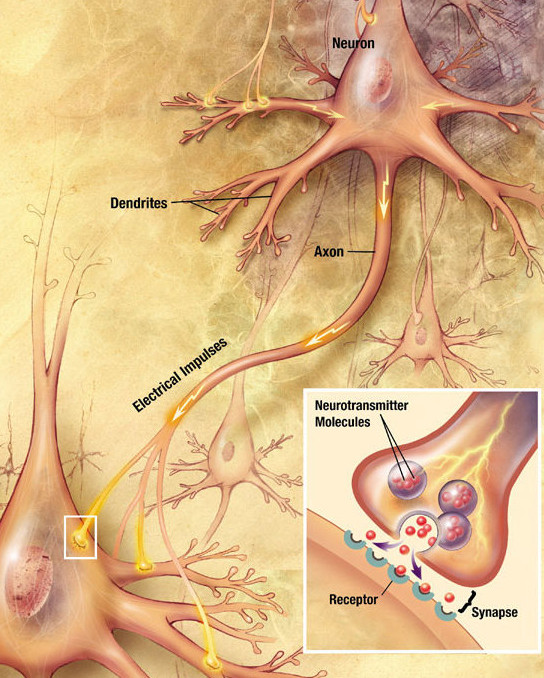
\includegraphics[width=0.3\textwidth]{synapse}
  \label{fig:synapse}
\end{SCfigure}

ANNs can be applied to all three broad machine learning categories: supervised (SL), unsupervised (UL) and reinforcement (RL). The most common is SL in which the expected output of the model is known and can be used to compare against and adjust the machine learning algorithm's hypothesis.  As sequence to sequence learning is an SL method, this discussion will be focused on the respective neural network algorithm. For more information on UL and RL, see~\cite{Becker1996} and~\cite{Sutton1998} respectively.

As mentioned previously, ANNs draw inspiration from biological neurons, containing an input layer, hidden layers, and an output later with numerous nodes in each. Every node, aside from those in the output, relays information to every other node in the proceeding network layer. These nodes simulate the neurons with connections between them representing axons and synapses.

\begin{figure}[h]
  \centering
  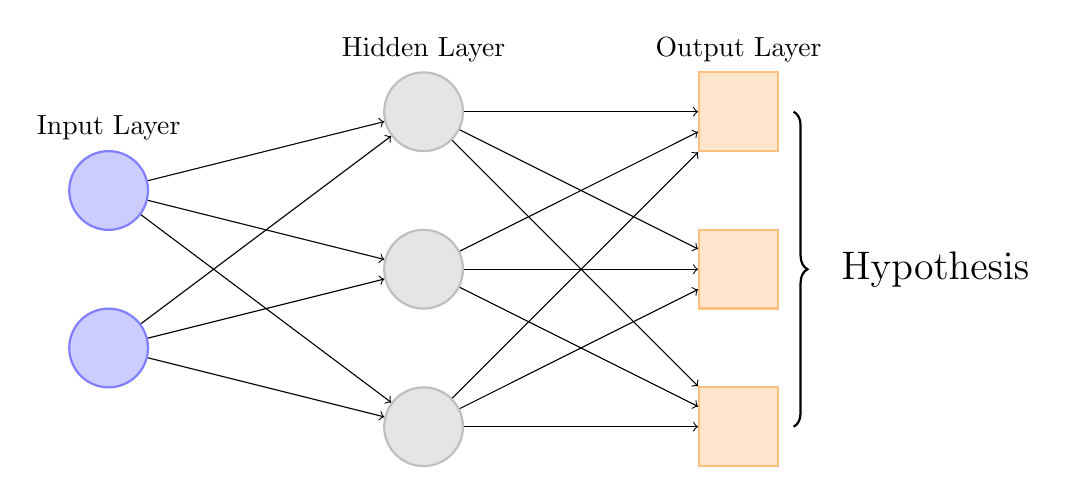
\begin{tikzpicture}
    \node[input] [label={Input Layer}] (input1) at (-4,1) {};
    \node[input] (input2) at (-4,-1) {};
    \node[hidden] [label={Hidden Layer}] (h1) at (0,2) {};
    \node[hidden] (h2) at (0,0) {};
    \node[hidden] (h3) at (0,-2) {};
    \node[output] [label={Output Layer}] (o1) at (4,2) {};
    \node[output] (o2) at (4,0) {};
    \node[output] (o3) at (4,-2) {};
    \node[minimum size = 20mm] (hyp) at (6.5,0) {\Large Hypothesis};
    \draw [->] (input1) to (h1);
    \draw [->] (input1) to (h2);
    \draw [->] (input1) to (h3);
    \draw [->] (input2) to (h1);
    \draw [->] (input2) to (h2);
    \draw [->] (input2) to (h3);
    \draw [->] (h1) to (o1);
    \draw [->] (h1) to (o2);
    \draw [->] (h1) to (o3);
    \draw [->] (h2) to (o1);
    \draw [->] (h2) to (o2);
    \draw [->] (h2) to (o3);
    \draw [->] (h3) to (o1);
    \draw [->] (h3) to (o2);
    \draw [->] (h3) to (o3);
    \draw[snake=brace,segment amplitude=5pt,thick] (4.7,2) -- (4.7,-2);
  \end{tikzpicture}

  \caption{A simple three layer neural network. NB: ANN Architectural naming convention is not entirely agreed upon, as found in~\cite{Fei-Fei2015}, but for the purposes of this review, we will consider all layers.}
  \label{fig:NNDiagram}
\end{figure}

In figure~\ref{fig:NNDiagram} above, a number of inputs from a single training example are  multiplied by a successive set of parameters, $\Theta^{(1)...(L)}$ where $L \in \R$ is number of layers in the network architecture, before being transformed by each neural node in each hidden layer to eventually arrive at an output, $y_{1...K}$ where K is the number of classifiers, called forward propagation (Sec.~\ref{fprop})~\cite{Ng2011a}. The model then calculates the amount of error between the calculated hypothesis based upon the parameter settings and the expected result (Sec.~\ref{costcalc}). The derivatives of these costs among all the hidden layers are calculated in a process called backward propagtion (Sec.~\ref{backprop}). These derivatives describe the angle of the error for each parameter and these errors are propagated backwards~\cite{Ng2011a}. A small change in the parameters designated by a learning rate, $\alpha$, and the severity of the error begins a process called gradient descent (Sec.~\ref{grad}) which will begin tuning the parameters.

This process is repeated for each training example in the dataset and iterated several times until the amount of error is no longer decreasing by a significant amount. Lastly, a new set of data with labels will be used to test the model. If the model has been tuned properly, it will ideally have a high degree of accurate predictions/classifications. If so, by backpropagating the errors, each layer has learned to recognise patterns, and even patterns within patterns. These four steps--Forward Propagation, Cost Calculation, Backward Propagation, and Gradient Descent--comprise the main components of a neural network and will now be explained in further detail.

\subsubsection{Forward Propagation}\label{fprop}
Before diving into the specifics, it is important to understand the terminology we will be using going forward. The inputs to a neural network are the attributes $x_i$ of the $i^{th}$ training example in the dataset, an $m \times n$ dimensional matrix containing all the testing data where $m$ is the number of training examples and $n$ is the number of attributes. Therefore, the amount of nodes, $j$, in the input layer will always equal $n$.

$l \in \R^L$ is the layer and will be superscripted and in parentheses. $i \ge1 \in \R^m$ is training example $i$. The weighted parameters $\Theta^{(l)}$ are an $j^{(l)} \times j^{(l+1)}$ dimensional matrix where $(l) \ge1 \in \R^L$\footnote{The referenced layer (l) will always be in parentheses to help distinguish it from the other dimensional attributes of the neural network} is the layer in the network. In other words, it has as many rows as the number of units in the layer passing the parameter and as many columns as the number of units in the next layer. There are as many $\Theta$s as there are hidden units plus the output layer. These matrices are randomly initialised to values near zero and are passed to the model.

The predicted output is referred to as $h_\Theta(x^{(i)})$, meaning the hypothesis given $\Theta$ as a function of training example $i$. The amount of output units is dependent upon the number of elements in the classifier.  For example, if the network is designed to distinguish between a picture of a dog, cat, mouse and tree, there will be four output units. The hypothesis will be a vector  assigning the probability the network predicts the image to be any of the given classifications.

Each of the neurons in the network will be referred to as activations, or $a_j^{(l)}$ where $j\ge1$ is the unit number in the network, starting from the top in figure~\ref{fig:fwdprop}. These activations multiply the output from each unit of the previous activation layer and $\Theta$ in a variable (\ref{eq:z}) and transform it using (\ref{eq:sig}).

\begin{align}
  z^{(l)} &= \Theta^{(l-1)}x^{(l-1)} \label{eq:z} \\ 
  g(z^{(l)}) &= \frac{1}{1+e^{-z^{(l)}}} \label{eq:sig} \\
  h_\Theta(x) &= g(z^{(L)})
\end{align}

\begin{figure}[h]\label{fig:fwdprop}
  \centering
  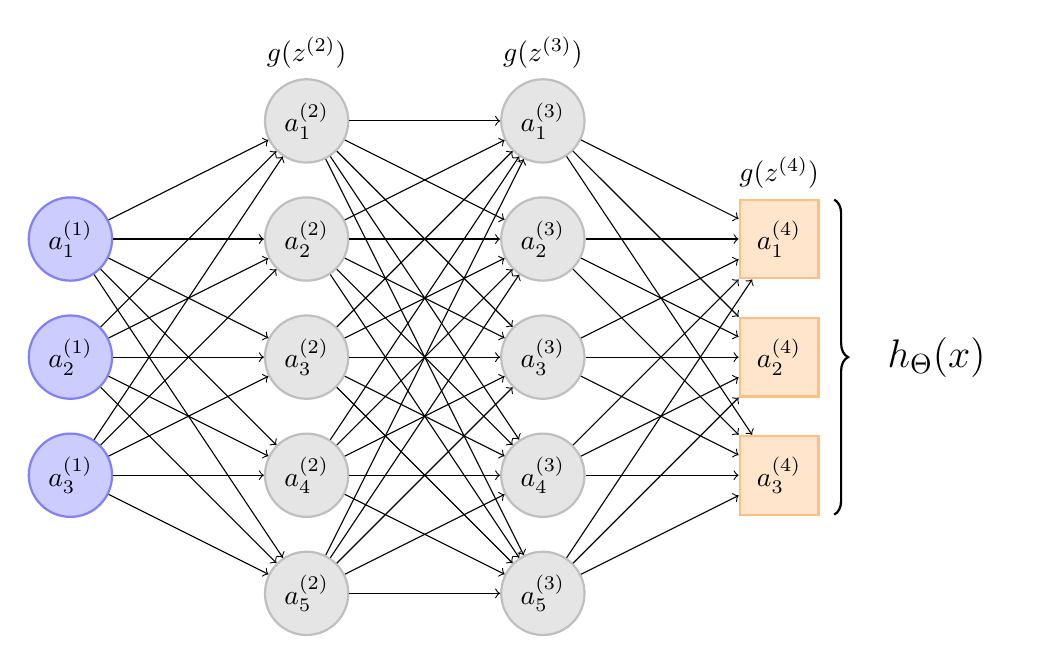
\begin{tikzpicture}
    % \newcommand{\iUnits}{3}
    % \newcommand{\hUnits}{5}
    % \newcommand{\oUnits}{3}
    \node[input] (input1) at (-3,1.5) {$a_1^{(1)}$};
    \node[input] (input2) at (-3,-0) {$a_2^{(1)}$};
    \node[input] (input3) at (-3,-1.5) {$a_3^{(1)}$};
    \node[hidden] [label=$g(z^{(2)})$] (h11) at (0,3) {$a_1^{(2)}$};
    \node[hidden] (h12) at (0,1.5) {$a_2^{(2)}$};
    \node[hidden] (h13) at (0,0) {$a_3^{(2)}$};
    \node[hidden] (h14) at (0,-1.5) {$a_4^{(2)}$};
    \node[hidden] (h15) at (0,-3) {$a_5^{(2)}$};
    \node[hidden] [label=$g(z^{(3)})$] (h21) at (3,3) {$a_1^{(3)}$};
    \node[hidden] (h22) at (3,1.5) {$a_2^{(3)}$};
    \node[hidden] (h23) at (3,0) {$a_3^{(3)}$};
    \node[hidden] (h24) at (3,-1.5) {$a_4^{(3)}$};
    \node[hidden] (h25) at (3,-3) {$a_5^{(3)}$};
    \node[output] [label=$g(z^{(4)})$] (o1) at (6,1.5) {$a_1^{(4)}$};
    \node[output] (o2) at (6,0) {$a_2^{(4)}$};
    \node[output] (o3) at (6,-1.5) {$a_3^{(4)}$};
    \node[minimum size = 20mm] (hyp) at (8,0) {\Large $h_\Theta(x)$};

    \draw [->] (input1) to (h11);
    \draw [->] (input1) to (h12);
    \draw [->] (input1) to (h13);
    \draw [->] (input1) to (h14);
    \draw [->] (input1) to (h15);
    \draw [->] (input2) to (h11);
    \draw [->] (input2) to (h12);
    \draw [->] (input2) to (h13);
    \draw [->] (input2) to (h14);
    \draw [->] (input2) to (h15);
    \draw [->] (input3) to (h11);
    \draw [->] (input3) to (h12);
    \draw [->] (input3) to (h13);
    \draw [->] (input3) to (h14);
    \draw [->] (input3) to (h15);
    
    \draw [->] (h11) to (h21);
    \draw [->] (h11) to (h22);
    \draw [->] (h11) to (h23);
    \draw [->] (h11) to (h24);
    \draw [->] (h11) to (h25);
    \draw [->] (h12) to (h21);
    \draw [->] (h12) to (h22);
    \draw [->] (h12) to (h23);
    \draw [->] (h12) to (h24);
    \draw [->] (h12) to (h25);
    \draw [->] (h13) to (h21);
    \draw [->] (h13) to (h22);
    \draw [->] (h13) to (h23);
    \draw [->] (h13) to (h24);
    \draw [->] (h13) to (h25);
    \draw [->] (h14) to (h21);
    \draw [->] (h14) to (h22);
    \draw [->] (h14) to (h23);
    \draw [->] (h14) to (h24);
    \draw [->] (h14) to (h25);
    \draw [->] (h15) to (h21);
    \draw [->] (h15) to (h22);
    \draw [->] (h15) to (h23);
    \draw [->] (h15) to (h24);
    \draw [->] (h15) to (h25);
    
    \draw [->] (h21) to (o1);
    \draw [->] (h21) to (o2);
    \draw [->] (h21) to (o3);
    \draw [->] (h22) to (o1);
    \draw [->] (h22) to (o2);
    \draw [->] (h22) to (o3);
    \draw [->] (h23) to (o1);
    \draw [->] (h23) to (o2);
    \draw [->] (h23) to (o3);
    \draw [->] (h24) to (o1);
    \draw [->] (h24) to (o2);
    \draw [->] (h24) to (o3);
    \draw [->] (h25) to (o1);
    \draw [->] (h25) to (o2);
    \draw [->] (h25) to (o3);

    \draw[snake=brace,segment amplitude=5pt,thick] (6.7,2) -- (6.7,-2);
  \end{tikzpicture}
  \caption{A neural network with two hidden layers and five activation units in each. Each training example has 3 attributes and there are four classifications for the output layer.}
\end{figure}

In figure~\ref{fig:fwdprop}, the input layer is a $3\times 1$ vector of the attributes of a single training example. To begin the forward propagation process, $\Theta^{(1)} \in \rdim{5}{3}$ is multiplied by the input vector (\ref{eq:z}), creating the vector $z^{(2)} \in \rdim{5}{1}$. This vector then gets transformed via the sigmoid function (\ref{eq:sig}). $\Theta^{(2)} \in \rdim{5}{5}$ is then multiplied by the resultant vector $a^{(2)} \in \rdim{5}{1}$ to obtain vector $z^{(3)} \in \rdim{5}{1}$.  The full chain of calculations can be seen in the following equations.
\begin{align*}
  a^{(1)} &= x \\
  z^{(2)} &= \Theta^{(1)}a^{(1)} \\
  a^{(2)} &= g(z^{(2)}) \\
  z^{(3)} &= \Theta^{(2)}a^{(2)} \\
  a^{(3)} &= g(z^{(3)}) \\
  z^{(4)} &= \Theta^{(3)}a^{(3)} \\
  a^{(4)} &= g(z^{(4)}) = h_\Theta(x)
\end{align*}

The result, $h_\Theta(x) \in \rdim{3}{1}$, is a vector of assigned probabilities for each classifier in the output. In the computer vision example from before, this would be with what certainty the model believed the image was a dog, cat, mouse or tree. Because each $\Theta$ is originally initialized randomly, the model's beginning hypotheses will be highly inaccurate, but once this error is calculated, we can begin the process of cost minimalisation, thereby improving, or training, the model.


\subsubsection{Cost Calculation} \label{costcalc}

Once the model has delivered an output $\hyp$, it will compare its results to the labeled results, $y$, a one-hot vector distinguishing which classifier was correct. In the case that a mouse, the third classifier, was correct, the vector would be $\begin{bmatrix} 0 & 0 & 1 & 0 \end{bmatrix}^T$. The hypotheses are compared to the labels to derive an overall cost for the network.  One of the most widely used cost functions is cross entropy\footnote{The reason for a logistic cost function has to do with convexity, a notorious problem for neural networks. It is beyond the scope of this literature review, but for more information, see~\cite{Nielsen2015}} (\ref{eq:cost}). The result of this cost function from each forward propagation will be a scalar that can be used to track progress during gradient descent (Sec.~\ref{grad}).

\begin{equation} \label{eq:cost}
  J(\Theta) = -\frac{1}{m}\sum_{i=1}^m\sum_{k=1}^K\left [y_k^{(i)}\log((h_\Theta(x^{(i)}))_k)+(1-y_k^{(i)})\log(1-(h_\Theta(x^{(i)}))_k)\right ]\underbrace{+\frac{\lambda}{2m}\sum_{l=1}^{L-1}\sum_{i=1}^{s_l}\sum_{j=1}^{s_{l+1}}(\Theta_{j,i}^{(l)})^2}_{Regularisation Parameter\footnote{The regularisation parameter is used to prevent overfitting the $\Theta$ values to the training data.  This is more of an implementation concern and not central to understanding ANNs. For more information, see~\cite{Nielsen2015}}}
\end{equation}

The cost, $J(\Theta)$, can be plotted on a multidimensional plot for various values of Theta within all the parameters. While the above network would have 65 dimensions, one for every tunable parameter within the three $\Theta$s, this is impossible to visualise. For simplicity we will consider two dimensions.

\begin{SCfigure}[1][h] \label{fig:grad}
  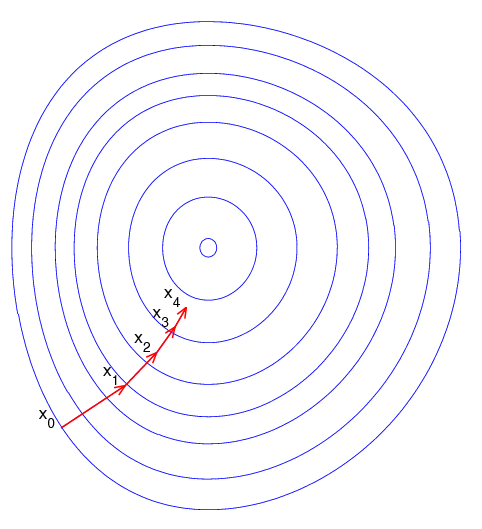
\includegraphics[scale=.25]{grad}
  \caption{A contour plot displaying gradient descent. From~\cite{pict}}
\end{SCfigure}

The first iteration of forward propagation will produce the error furthest from the minimum. We can measure the angle of the slope of the error (Sec.~\ref{backprop}) and take steps towards the minimum (Sec.\ref{grad}).

\subsubsection{Backward Propagation} \label{backprop}
Backpropagation can be thought of simply as the chain rule in calculus\footnote{For information on this, see~\cite{Thomas2002}} via matrix multiplication.  Consider the graph from Sec.~\ref{fprop} but with the direction reversed (Figure~\ref{backprop}).
\begin{figure}[h!] \label{fig:backprop}
  \centering
  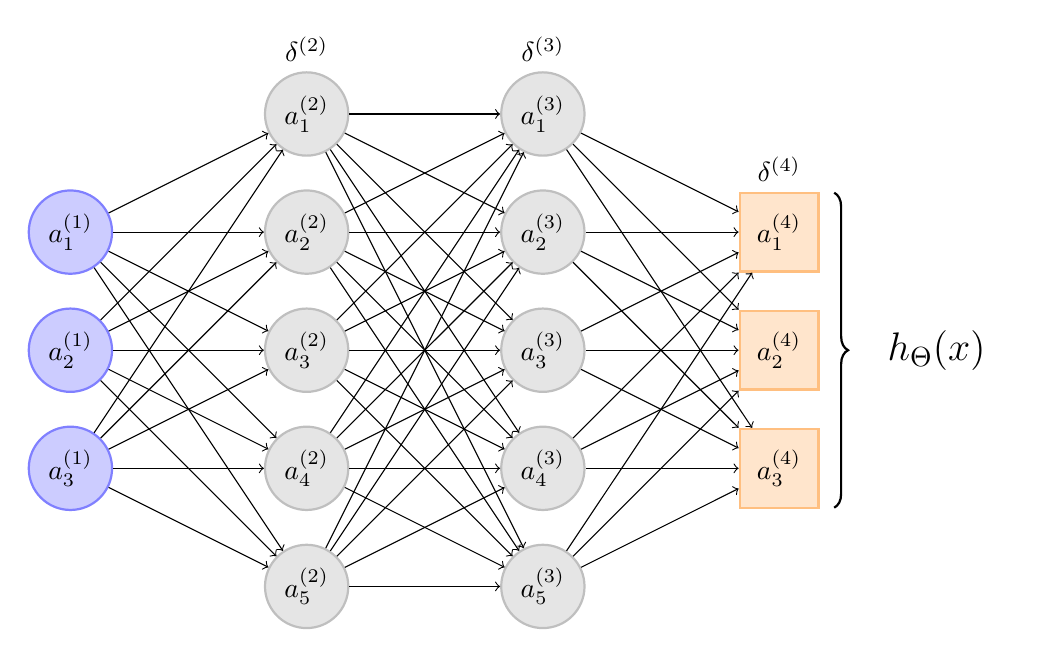
\begin{tikzpicture}
    \node[input] (input1) at (-3,1.5) {$a_1^{(1)}$};
    \node[input] (input2) at (-3,-0) {$a_2^{(1)}$};
    \node[input] (input3) at (-3,-1.5) {$a_3^{(1)}$};
    \node[hidden] [label=$\delta^{(2)}$] (h11) at (0,3) {$a_1^{(2)}$}
    edge [pre] (input1)
    edge [pre] (input2)
    edge [pre] (input3);
    \node[hidden] (h12) at (0,1.5) {$a_2^{(2)}$}
    edge [pre] (input1)
    edge [pre] (input2)
    edge [pre] (input3);
    \node[hidden] (h13) at (0,0) {$a_3^{(2)}$}
    edge [pre] (input1)
    edge [pre] (input2)
    edge [pre] (input3);
    \node[hidden] (h14) at (0,-1.5) {$a_4^{(2)}$}
    edge [pre] (input1)
    edge [pre] (input2)
    edge [pre] (input3);
    \node[hidden] (h15) at (0,-3) {$a_5^{(2)}$}
    edge [pre] (input1)
    edge [pre] (input2)
    edge [pre] (input3);
    \node[hidden] [label=$\delta^{(3)}$] (h21) at (3,3) {$a_1^{(3)}$}
    edge [pre] (h11)
    edge [pre] (h12)
    edge [pre] (h13)
    edge [pre] (h14)
    edge [pre] (h15);
    \node[hidden] (h22) at (3,1.5) {$a_2^{(3)}$}
    edge [pre] (h11)
    edge [pre] (h12)
    edge [pre] (h13)
    edge [pre] (h14)
    edge [pre] (h15);
    \node[hidden] (h23) at (3,0) {$a_3^{(3)}$}
    edge [pre] (h11)
    edge [pre] (h12)
    edge [pre] (h13)
    edge [pre] (h14)
    edge [pre] (h15);
    \node[hidden] (h24) at (3,-1.5) {$a_4^{(3)}$}
    edge [pre] (h11)
    edge [pre] (h12)
    edge [pre] (h13)
    edge [pre] (h14)
    edge [pre] (h15);
    \node[hidden] (h25) at (3,-3) {$a_5^{(3)}$}
    edge [pre] (h11)
    edge [pre] (h12)
    edge [pre] (h13)
    edge [pre] (h14)
    edge [pre] (h15);
    \node[output] [label=$\delta^{(4)}$] (o1) at (6,1.5) {$a_1^{(4)}$}
    edge [pre] (h21)
    edge [pre] (h22)
    edge [pre] (h23)
    edge [pre] (h24)
    edge [pre] (h25);
    \node[output] (o2) at (6,0) {$a_2^{(4)}$}
    edge [pre] (h21)
    edge [pre] (h22)
    edge [pre] (h23)
    edge [pre] (h24)
    edge [pre] (h25);
    \node[output] (o3) at (6,-1.5) {$a_3^{(4)}$}
    edge [pre] (h21)
    edge [pre] (h22)
    edge [pre] (h23)
    edge [pre] (h24)
    edge [pre] (h25);
    \node[minimum size = 20mm] (hyp) at (8,0) {\Large $h_\Theta(x)$};
    \draw[snake=brace,segment amplitude=5pt,thick] (6.7,2) -- (6.7,-2);
  \end{tikzpicture}
  \caption{Notice the arrows are pointed in the opposite direction.}
\end{figure}

In order to minimise the error, we take the derivative (\ref{derive}) of the cost function (\ref{costfunc}) and compute the error.  In other words, $\delta_j^{(l)}$ is the ``error'' of cost for $a_j^{(l)}$ (unit $j$ in layer $l$)~\cite{Ng2011a}.

\begin{align}
  \delta_j^{(l)} &= \frac{\partial}{\partial z_j^{(l)}} \text{cost ($i$), where} \label{derive}\\
  \text{cost}(i) &= y^{(i)}\log h_\Theta(x^{(i)})+(1-y^{(i)})\log h_\Theta(x^{(i)}) \label{costfunc}
\end{align}

The chain of derivatives is shown below. The derivative of the sigmoid is not shown and left as an exercise to the reader. The solutions can be found in~\cite{Ng2011a}.

\begin{align*}
  \delta^{(4)} &= a^{(4)} - y_i \\
  \delta^{(3)} &= (\Theta^{(3)})^T \delta_j^{(4)} \odot g'(z^{(3)}) \\
  \delta^{(2)} &= (\Theta^{(2)})^T \delta_j^{(4)} \odot g'(z^{(2)}) \\
\end{align*}
Notice that there is no $\delta^{(1)}$. This would correspond to the input layer, the vector of original attributes in the training data. Consequently, these can have no error~\cite{Ng2011a}. The errors for each layer of every node of every training example are then accumulated in matrices $\Delta^{(l)} \in \rdim{(l)}{(l+1)}$ (\ref{DeltaEQ}) for each training example. Note that each $\Delta$ contains the same dimensions as its corresponding $\Theta^{(l)}$, which makes intuitive sense as $\Delta^{(l)}$ is tracking the error caused by $\Theta^{(l)}$. Accordingly, there will be the same number of $\Delta$s and later $D$ (Sec.~\ref{grad}) as there are $\Theta$s.

\begin{equation} \label{DeltaEQ}
  \Delta_{i,j}^{(l)} := \Delta_{i,j}^{(l)} + a_j^{(l)}\delta_i^{(l+1)}
\end{equation}

Intuitively, this is multiplying the result of the activation of each node in layer $l$  by the amount of error it caused in the proceeding layer. The errors from each training example are continually added to the same $\Delta_{i,j}^{(l)}$ until the entire training set has been both forward and backward propagated, at which point gradient descent is implemented.

\subsubsection{Gradient Descent} \label{grad}
Once all the errors for every training example have been accumulated and back propagation has been completed, gradient descent must be implemented. To complete the derivative calculation for error minimisation, $D \in \rdim{j}{l}$,the completed $\Delta$ is divided by the number of training examples to achieve an average over the training set.
\begin{align*}
  D_{i,j}^{(l)} &:= \frac{1}{m}\Delta_{(i,j)}^{(l)}+\underbrace{\lambda \Theta_{(i,j)}^{(l)}}_{Regularisation\footnotemark} \\
  D_{i,j}^{(l)} &= \D
\end{align*}

\addtocounter{footnote}{-1}
\footnotetext{See footnote for equation (\ref{eq:cost})}

Now that the final derivative $D$ has been calculated, each $\Theta$ needs to be reassigned to a new value that will produce an error closer to the local minimum (\ref{reassign}). The learning rate, $\alpha$ is a parameter set by the ANN designer to control how large each step of gradient descent is. If this rate is too large, the ANN will never reach the local minimum as it will overshoot it as it gets closer.  If it is too small, the ANN will take much longer to train.

\begin{equation} \label{reassign}
  Theta^{(l)} = \Theta^{(l)} + \alpha\D
\end{equation}

This marks the completion of one full pass of a neural network.  It has started to learn parameters and the more iterations that are done, the closer the neural network will come to minimizing the error function, fine tuning the $\Theta$s at every step. Once this ANN has been completed, it should produce a high degree of accuracy in its classification task.

\subsubsection{Conclusion}
There are many types of ANN, and this was just an example of a simple classifying feedforward neural network (FNN). FNNs, also known as acyclic~\cite{Schmidhuber2015}, have no preservation of previous states. Once a pass through the network has completed, it has no impact on the next result. This is beneficial for certain tasks such as static image recognition, but what if you wanted a machine to predict what was going to happen next in a video given sufficient context, or generate grammatically correct sentences? Without any influence from previous passes through the network, no context can be developed and so FNNs are poorly suited to sequential tasks~\cite{LeCun2015,Schmidhuber2015}. While LSTMs (Sec.~\ref{LSTM}) are the defacto algorithms used to address this problem today~\cite{Schmidhuber2015}, they are only a modified version of a classical RNN~\cite{Hochreiter1997}, so understanding RNNs will help in understanding the more complex LSTMs.

\subsection{Recurrent Neural Networks}\label{RNN}

\subsection{Long Short-Term Memory}\label{LSTM}

\subsection{Sequence-to-Sequence Learning}\label{S2S}
\section{Methodology}\label{methodology}

To construct the initial seq2seq model, the PyTorch neural network library for python was used. Recall from Section~\ref{tf} that other state-of-the-art solutions are not able to implement dynamic teacher forcing methods due to the fact that the computational graph must be pre-defined before inference. 

Specifically, I used an open source seq2seq pytorch jupyter notebook for neural machine translation\footnote{Available at: https://github.com/jph00/part2/blob/master/translate-pytorch.ipynb} as the base model. Several modifications were made to this model, including the implementation of bidirectional RNNs and various teacher forcing methods, as well as redefining input and output parameters for the specific task of headline-length abstractive summarization.

\subsection{Data and Preprocessing}
The dataset used for this project and all other state-of-the-art models for this task is The University of Pennsylvania Linguistic Data Consortium's Annotated English Gigaword Corpus\footnote{https://catalog.ldc.upenn.edu/ldc2012t21}, graciously provided via scholarship, which contains over four million article-headline pairs from seven news publications between 1994 to 2010. Specifically, the LDC data was structured as 1,011 gzipped XML files, each file representing a month of articles from one of the news sources. Because the data was delivered via an external hard drive and I did not have access to a University computer, the dataset had to be processed on a 2015 Macbook Pro. Unfortunately, this meant that the 154 largest XML files had to be discarded due to the computers inability to store their parsed XML trees in memory. It was decided that the dataset should be pared back to \~100,000 pairs, so 120 articles were sampled randomly from each of the remaining 857 files.

To address the file format, the LXML library was used to unzip and parse the XML tree. After randomly shuffling all of the child nodes of the XML tree, a series of regex substitutions were used to strip the unnecessary part-of-speech tags which accompanied every word in the dataset to transform the necessary data into raw text. It must be noted that all state-of-the-art headline generation models currently only use the first sentence of the article as input, as this is generally found to be sufficient to generate headlines~\cite{Liu2016}. I maintained this convention within this project, so any reference to an article is only to the first sentence of said article in practice.

One drawback of the LDC dataset is that there is a non-negligable amount of nonsensical headlines that also happen to be very long. To combat this, I restricted the length of headlines to 30 words and articles to a length of 50 words, the same criteria used in the highest-performing model~\cite{Liu2016}. Any pairs that did not meet both of these criteria were discarded, resulting in a 20.7\% discard rate. The remaining 79.3\% randomly sampled, fully preprocessed article/headline pairs were then placed into respective lists. The code for extracting the data can be found in Appendix~\ref{app:extraction}.

The sentences were then turned into word indexes within a vocabulary list for every headline/article pair, keeping the 200,000 most common words and substituting all other words with an $<UNK>$ token, for unknown. This practice is in line with the highest-performing state-of-the-art model~\cite{Liu2016}. A $<SOS>$, start of sentence pad, or index 1, was added to the start of every pair. Then each sentence was padded with the $<PAD>$ token, or index 0, on the ends to make each input and output the same length. The data was then split 90\% training, 10\% test. Lastly, each word was also linked with its associated 100-dimensional GLoVe embedding (See Sec.~\ref{emb}) if an embedding existed for the word. Otherwise, a random initialization was created for the word to be trained by the model. Unfortunately, due to licensing constraints, I cannot share the contents of any of the data, but the processed, indexed pairs can be seen in Figure~\ref{fig:procd}.

\begin{figure}[h]
  \centering
  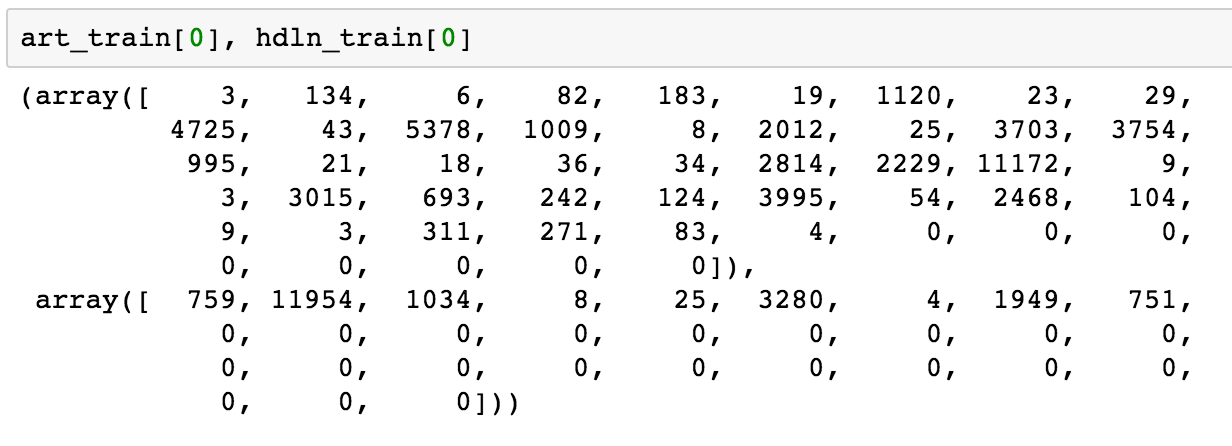
\includegraphics[width=.85\textwidth]{procd}
  \caption{A preprocessed headline and article pair with zero-padding.}
  \label{fig:procd}
\end{figure}

\subsection{Difficulties and RNN Architecture Adjustments}
When initially setting out to research this issue of teacher forcing, several large issues presented themselves. First and foremost, training DNNs can take significant resources, some using more than 300 GPUs simultaneously~\cite{Silver2016}. For my specific task,attempts at adhereing to state-of-the-art model parameters revelaed that fully training such a model from scratch would take over 10 days per experiment on a single GPU, confirmed by~\cite{Nallapati2016a}. Furthermore, because teacher forcing is a method used during model training, pretrained models could not be used. Therefore, modifications were required to achieve results within a reasonable time.

The current state-of-the-art headline generation model uses four bidirectional encoder layers, four bidirectional decoder layers, a word embedding size of 128, and 256 hidden nodes per LSTM~\cite{Liu2016}. The greater one can increase any of these dimensions, the greater the model's learned complexities between inputs, outputs and intra-word relationships at the cost of computational requirement for both training and evaluating. This model was trained on multiple GPUs (though the exact number is not specified) and appeared that it would take weeks to converge on a single GPU through a short test run. Because of this, the same general seq2seq architecture was maintained, but all dimensionalities reduced to the following: one layer encoder, one layer decoder, word embedding size of 300, and hidden size of 128 nodes per LSTM. With these parameters, models appear to converge within approximately four hours on the University's Titan X (Pascal) GPU instance (Thadeus machine). Due to this decrease in model complexity, one cannot hope for comparative results to state-of-the-art, so instead, results for various teacher forcing methods will only be judged relative to one another.

As a final precaution, it must be noted that these models are learning sequence generation from headlines that have been chosen by the publications, meaning they are still subject to bias. The idea, however, is that by generalizing well enough amongst a large dataset, biases will naturally be mitigated. I think this is likely incorrect, and that Recurrent Neural Networks will pick up trace biases by the very nature of their capability to understand and interpret nuance to such an incredible degree of dimensionality. That said, developing effective abstractive techniques is the first step in a long road towards the mitigation of editorial bias in online news, and seq2seq is currently at the forefront of development in this arena.

\subsection{Experiment Set-up}
Recall from Section~\ref{grad} that a learning rate is picked by the DNN engineer to change all the weights within the network. This learning rate needs to be decreased as the model gets closer and closer to convergence in a process called learning rate annealing. It was found that 40,000 cycles of generating a random batch of 128 examples, annealed every 5,000 - 10,000 cycles, was adequate for model convergence. The first two sets of 5,000 batches had a learning rate of 0.003; the second two sets of 5,000 had learning rates of 0.001; the third two sets of 5,000 batches had learning rates of 0.0003; the next set of 5,000 had a learning rate of 0.0001; the last set of 5,000 had a learning rate of 0.00003. This progression can be seen clearly in the \texttt{multi\_train} function in Appendix~\ref{app:train}.

I trained seven different models on these teacher forcing (TF) methods: graduated, graduated-reset, 100\%, 75\%, 50\%, 25\%, and 0\%. For the graduated model, the chance of teacher forcing started at 100\% and decreased linearly over the course of the entire 40,000 batches of training until eventually 0\% teacher forcing was allowed by the last batch. Graduated-reset would gradually decrease the amount of teacher forcing over every 5,000 batches, so full teacher forcing was reset to 100\% and tapered to 0\% for each of the 8 sets of 5,000 batches. The differences can be further investigated by referencing the \texttt{trainEpochs} and \texttt{fullgraduated\_trainEpochs} functions in Appendix~\ref{app:train}. The various percentages listed above provided the associated teacher forcing probability throughout the entire training period.

To ensure that the training and test splits were not disproportionately influencing one TF method over another by chance, I trained and tested every model 3 different times on randomized data splits. In doing so, I was able to ascertain that all TF methods on all three tests were statistically similar, and consequently any of the test results could be used for further analysis. See Section~ref{stat} for details.

\subsection{Evaluation Metrics}
When evaluating the effectiveness of various teacher forcing methods, there are two main metrics to condiser: loss over time and ROUGE.

\subsubsection{ROUGE}\label{method:rouge}
Firstly, to judge generative performance, the metric used in all previous explorations of headline-length text summarization~\cite{Rush2015,Chopra2016,Nallapati2016a,Liu2016,See2017}: Recall-Oriented Understudy for Gisting Evaluation, or ROUGE~\cite{Lin2004}, will likewise be used for this project. There are two ROUGE metrics of interest: ROUGE-1, ROUGE-2. For the purposes of this task, ROUGE-1 measures the overlap of each word between the generated summary and the label. ROUGE-2 measures the overlap of adjacent words between the generated summary and the correct label. The top ROUGE scores for each state-of-the-art abstractive model can be compared in Table~\ref{tab:rouge}.
\begin{table}[h]
  \begin{center}
    \begin{tabular}{ | l l | c | c | }
      \hline
      & & ROUGE-1 & ROUGE-2 \\
      \hline
      Rush & [Facebook] & 29.78 & 11.89 \\
      Chopra & [Facebook] & 33.78 & 15.97 \\
      Nallapati & [IBM] & 35.30 & 16.64 \\
      Liu & [Google Brain] & 42.56 & 23.12 \\
      \hline
    \end{tabular}
    \caption{ROUGE-1 and ROUGE-2 scores for top performing abstractive models}
    \label{tab:rouge}
  \end{center}
\end{table}
By measuring these values, we can ascertain how close the generated output was to matching words and word pairs from the beginning. While this metric is quite unsophisticated and does not well convey actual comprehension, it is the metric used by all other headline-length abstractive summarization researchers to judge performance and consequently is the metric chosen to be used here.

\subsubsection{Loss Over Time}
Evaluating visualizations of loss over the training period is another important metric in judging the effectiveness of various TF methods. Recall from Section~\ref{tf} that the reason teacher forcing became a topic of discussion in the first place was the idea that, at the beginning of model training, the model would be generating the wrong output nearly every time. If this incorrect output was constantly fed into the decoder state to predict the next time step, all training afterwards is unhelpful. This would result in far longer convergence times. So, the amount of time it takes for a model to converge is a critical part of the motivation behind teacher forcing. Consequently, the average loss over time was recorded and used to compare the various teacher forcing techniques.

\subsection{Statistical Analysis and Data Visualization}\label{stat}
To compare and contrast the results of the various TF methods from the three different tests, I used the Kruskal-Wallis Test~\cite{Kruskal1952}, which tests whether a number of samples are statistically probable to originate from the same distribution. These results can be found in Section~\ref{results}. As all TF methods over all three tests returned probable to have come from the same distribution, it is safe to assume that all TF methods from all three tests are representative of a general trend, and consequently further analysis only needed to be carried out on one of the tests. To visualize the skewed ROUGE distributions, I created histograms and Q-Q plots using R.

For computing average ROUGE values, I could not discern the methodology used by any of the state-of-the-art researchers. As such, I used what I felt was appropriate given the data distribution. That said, for skewed datasets, the median is typically used and was initially attempted for this analysis. However, the Wilcoxon pseudo-median values gave wildly inaccurate results for ROUGE-2. It would appear that non-normal median-distributed data was not properly accounting for ROUGE values of zero, a statistic that is very important to this specific problem. Consequently, bootstrapping~\cite{Davidson2003}, a mean-centric resampling technique, was used to compute these averages instead.

To test for statistically significant differences between the data, the Wilcoxon test~\cite{Wilcoxon1945} was used. This is a method used for paired difference testing on non-normal data distributions. The values reported are probabilities (p-values) that the differences in median of the compared TF methods is 0. This means that smaller p-values make it less of a possibility that the compared means are in fact the same and no statistical significance exists between them. A p-value $\leq$ 0.05 (5.0E-02) makes the differences statistically significant. Wilcoxon probabilities were calculated relative to three different benchmarks:  all TF methods relative to no TF, all TF methods relative to 100\% TF, and graduated compared to reset-graduated as a matter of academic interest.

Lastly, a look at loss over time is done as a second evaluation metric, again with only one of the test results. The loss and time information was collected in lists during training. These were then plotted using matplotlib, a MATLAB-esque plotting program for python and heavily used in jupyter notebooks. These plots have been provided in Section~\ref{loss}.
\section{Results}\label{results}
After running all seven teacher forcing methods 3 times each, the results for each TF method across the different tests were compared using Kruskal-Wallis, as described in Section~\ref{stat}. 

\subsection{ROUGE Scores}\label{results:rouge}
Before diving into ROUGE scores, it is important to understand the distributions of the ROUGE scores for the purposes of statistical analysis. The data is right (positively) skewed, as visualized in Figures~\ref{fig:r1hists}~and~\ref{fig:r2hists}.

\begin{figure}[h]
  \centering
  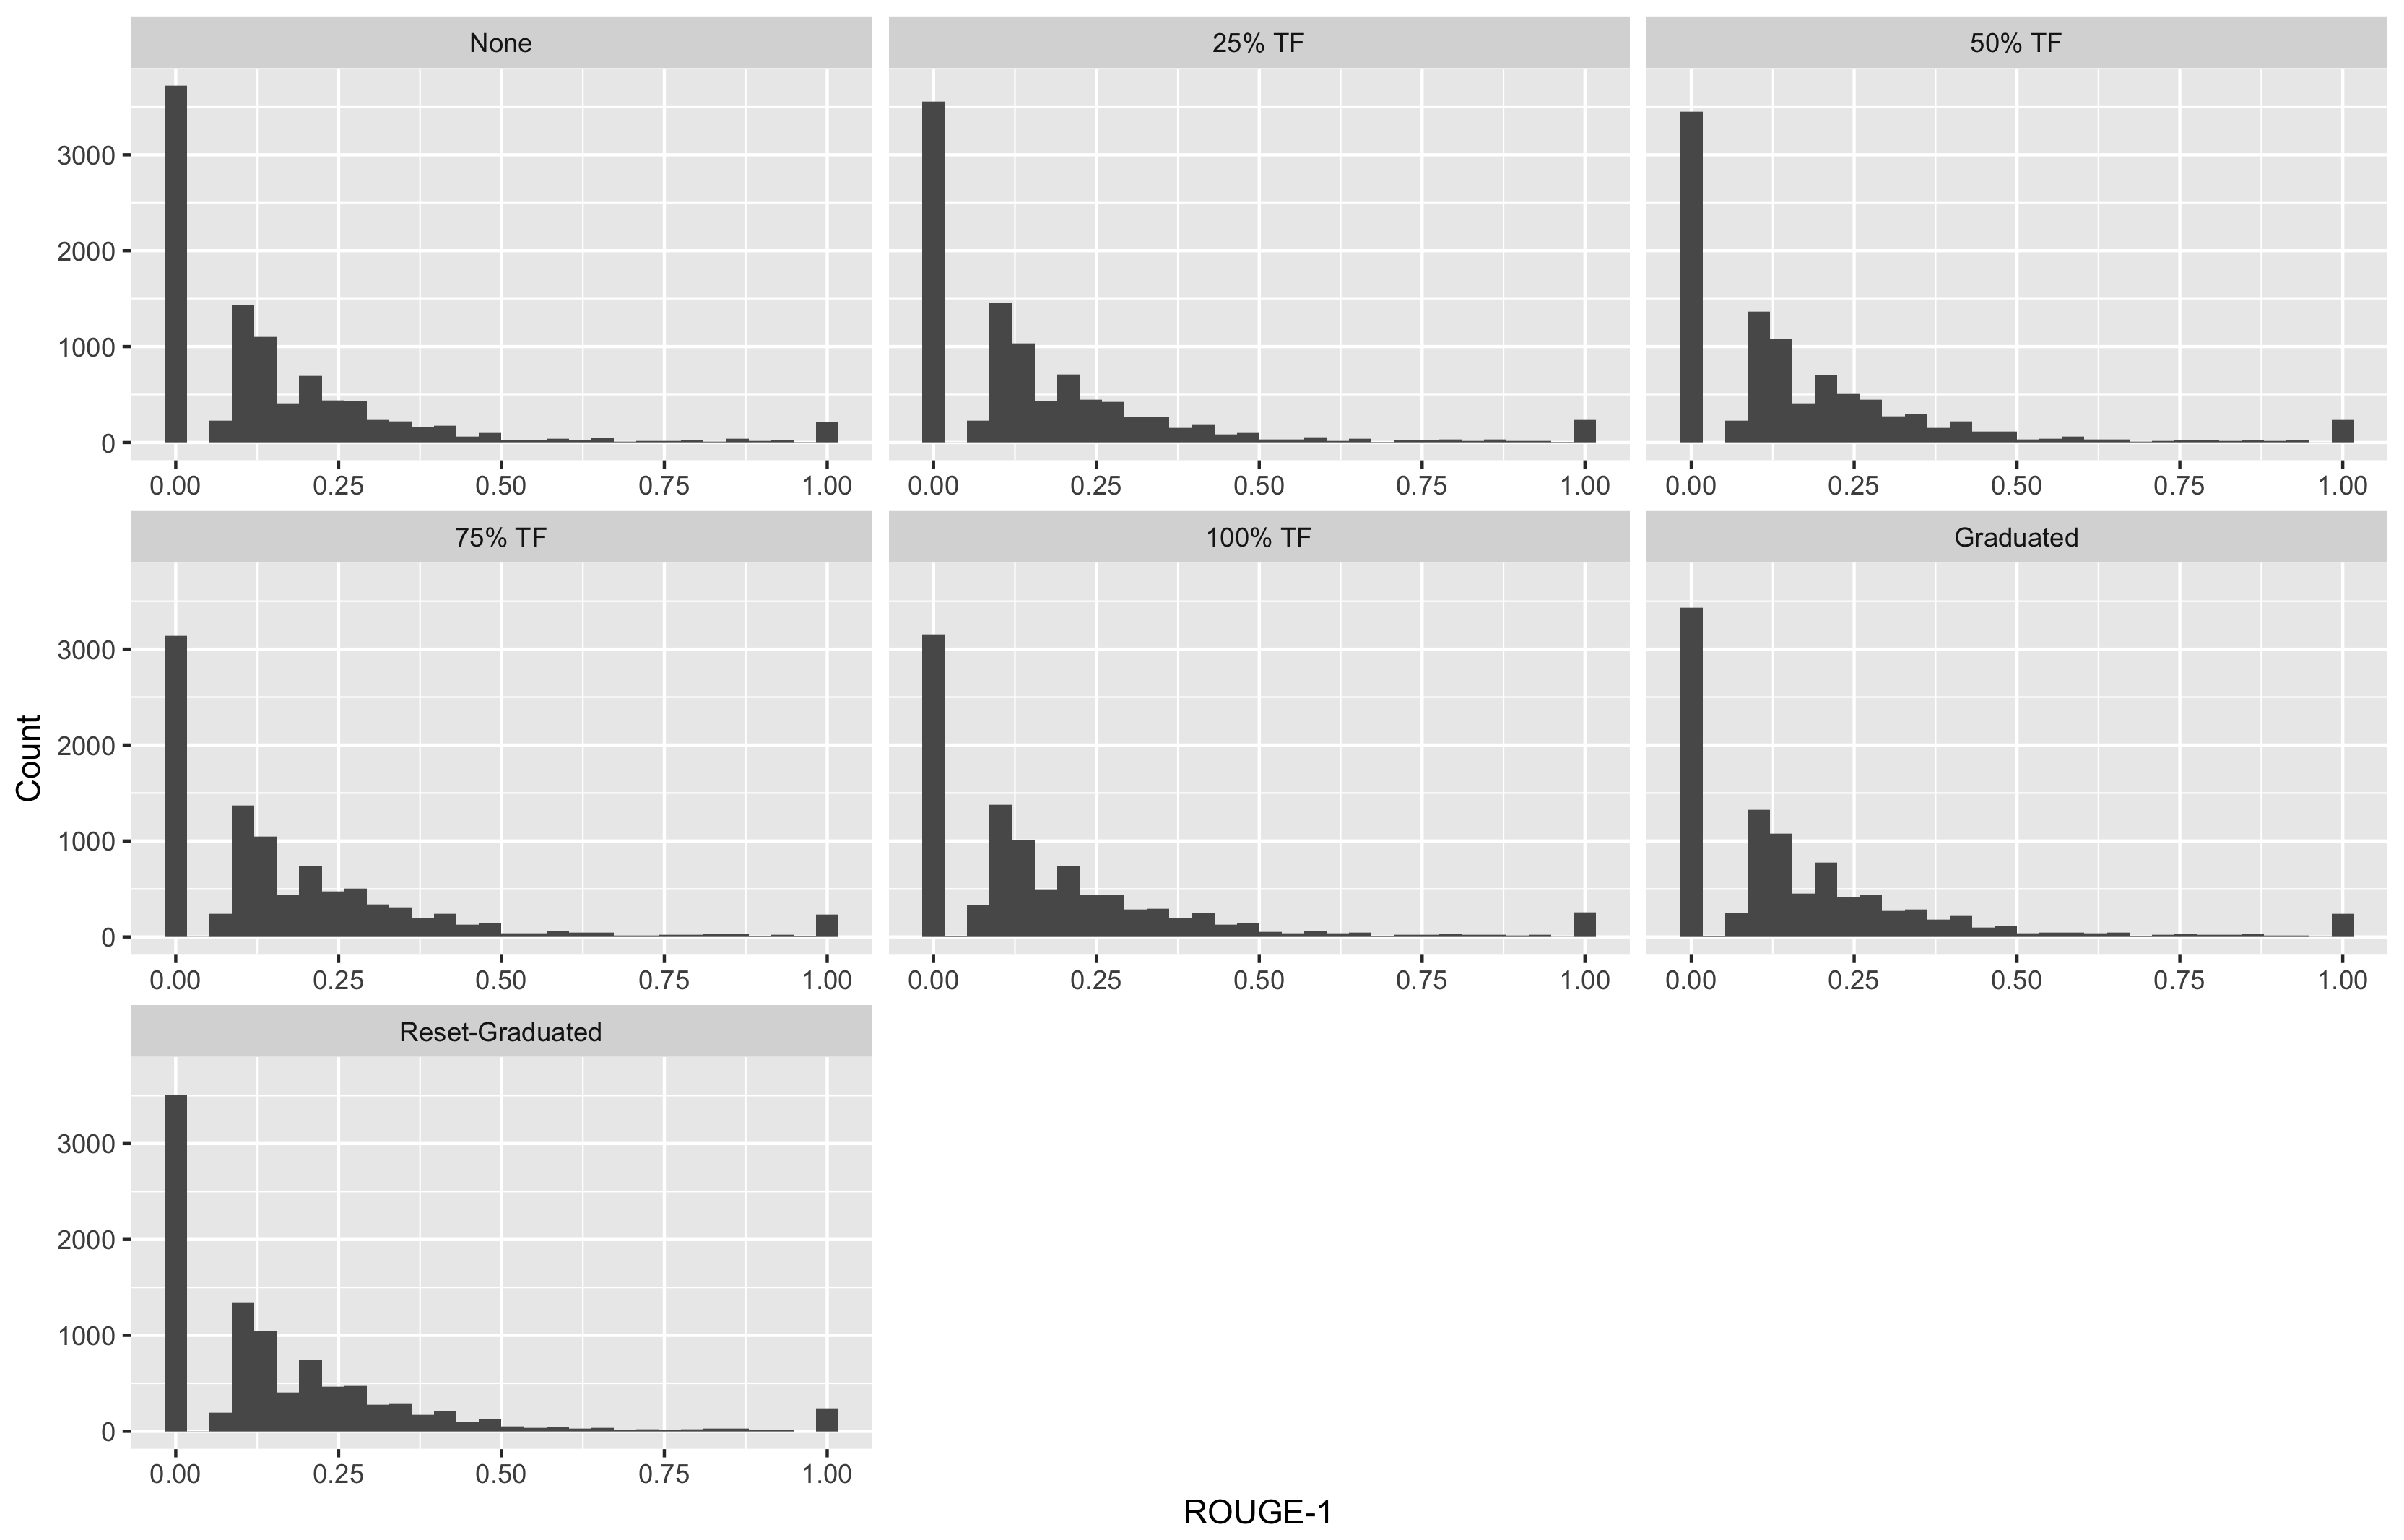
\includegraphics[width=0.8\textwidth]{../plots/test2/r1hists}
  \caption{Histograms of ROUGE-1 scores from all TF methods of Test 2}
  \label{fig:r1hists}
\end{figure}

\begin{figure}[h]
  \centering
  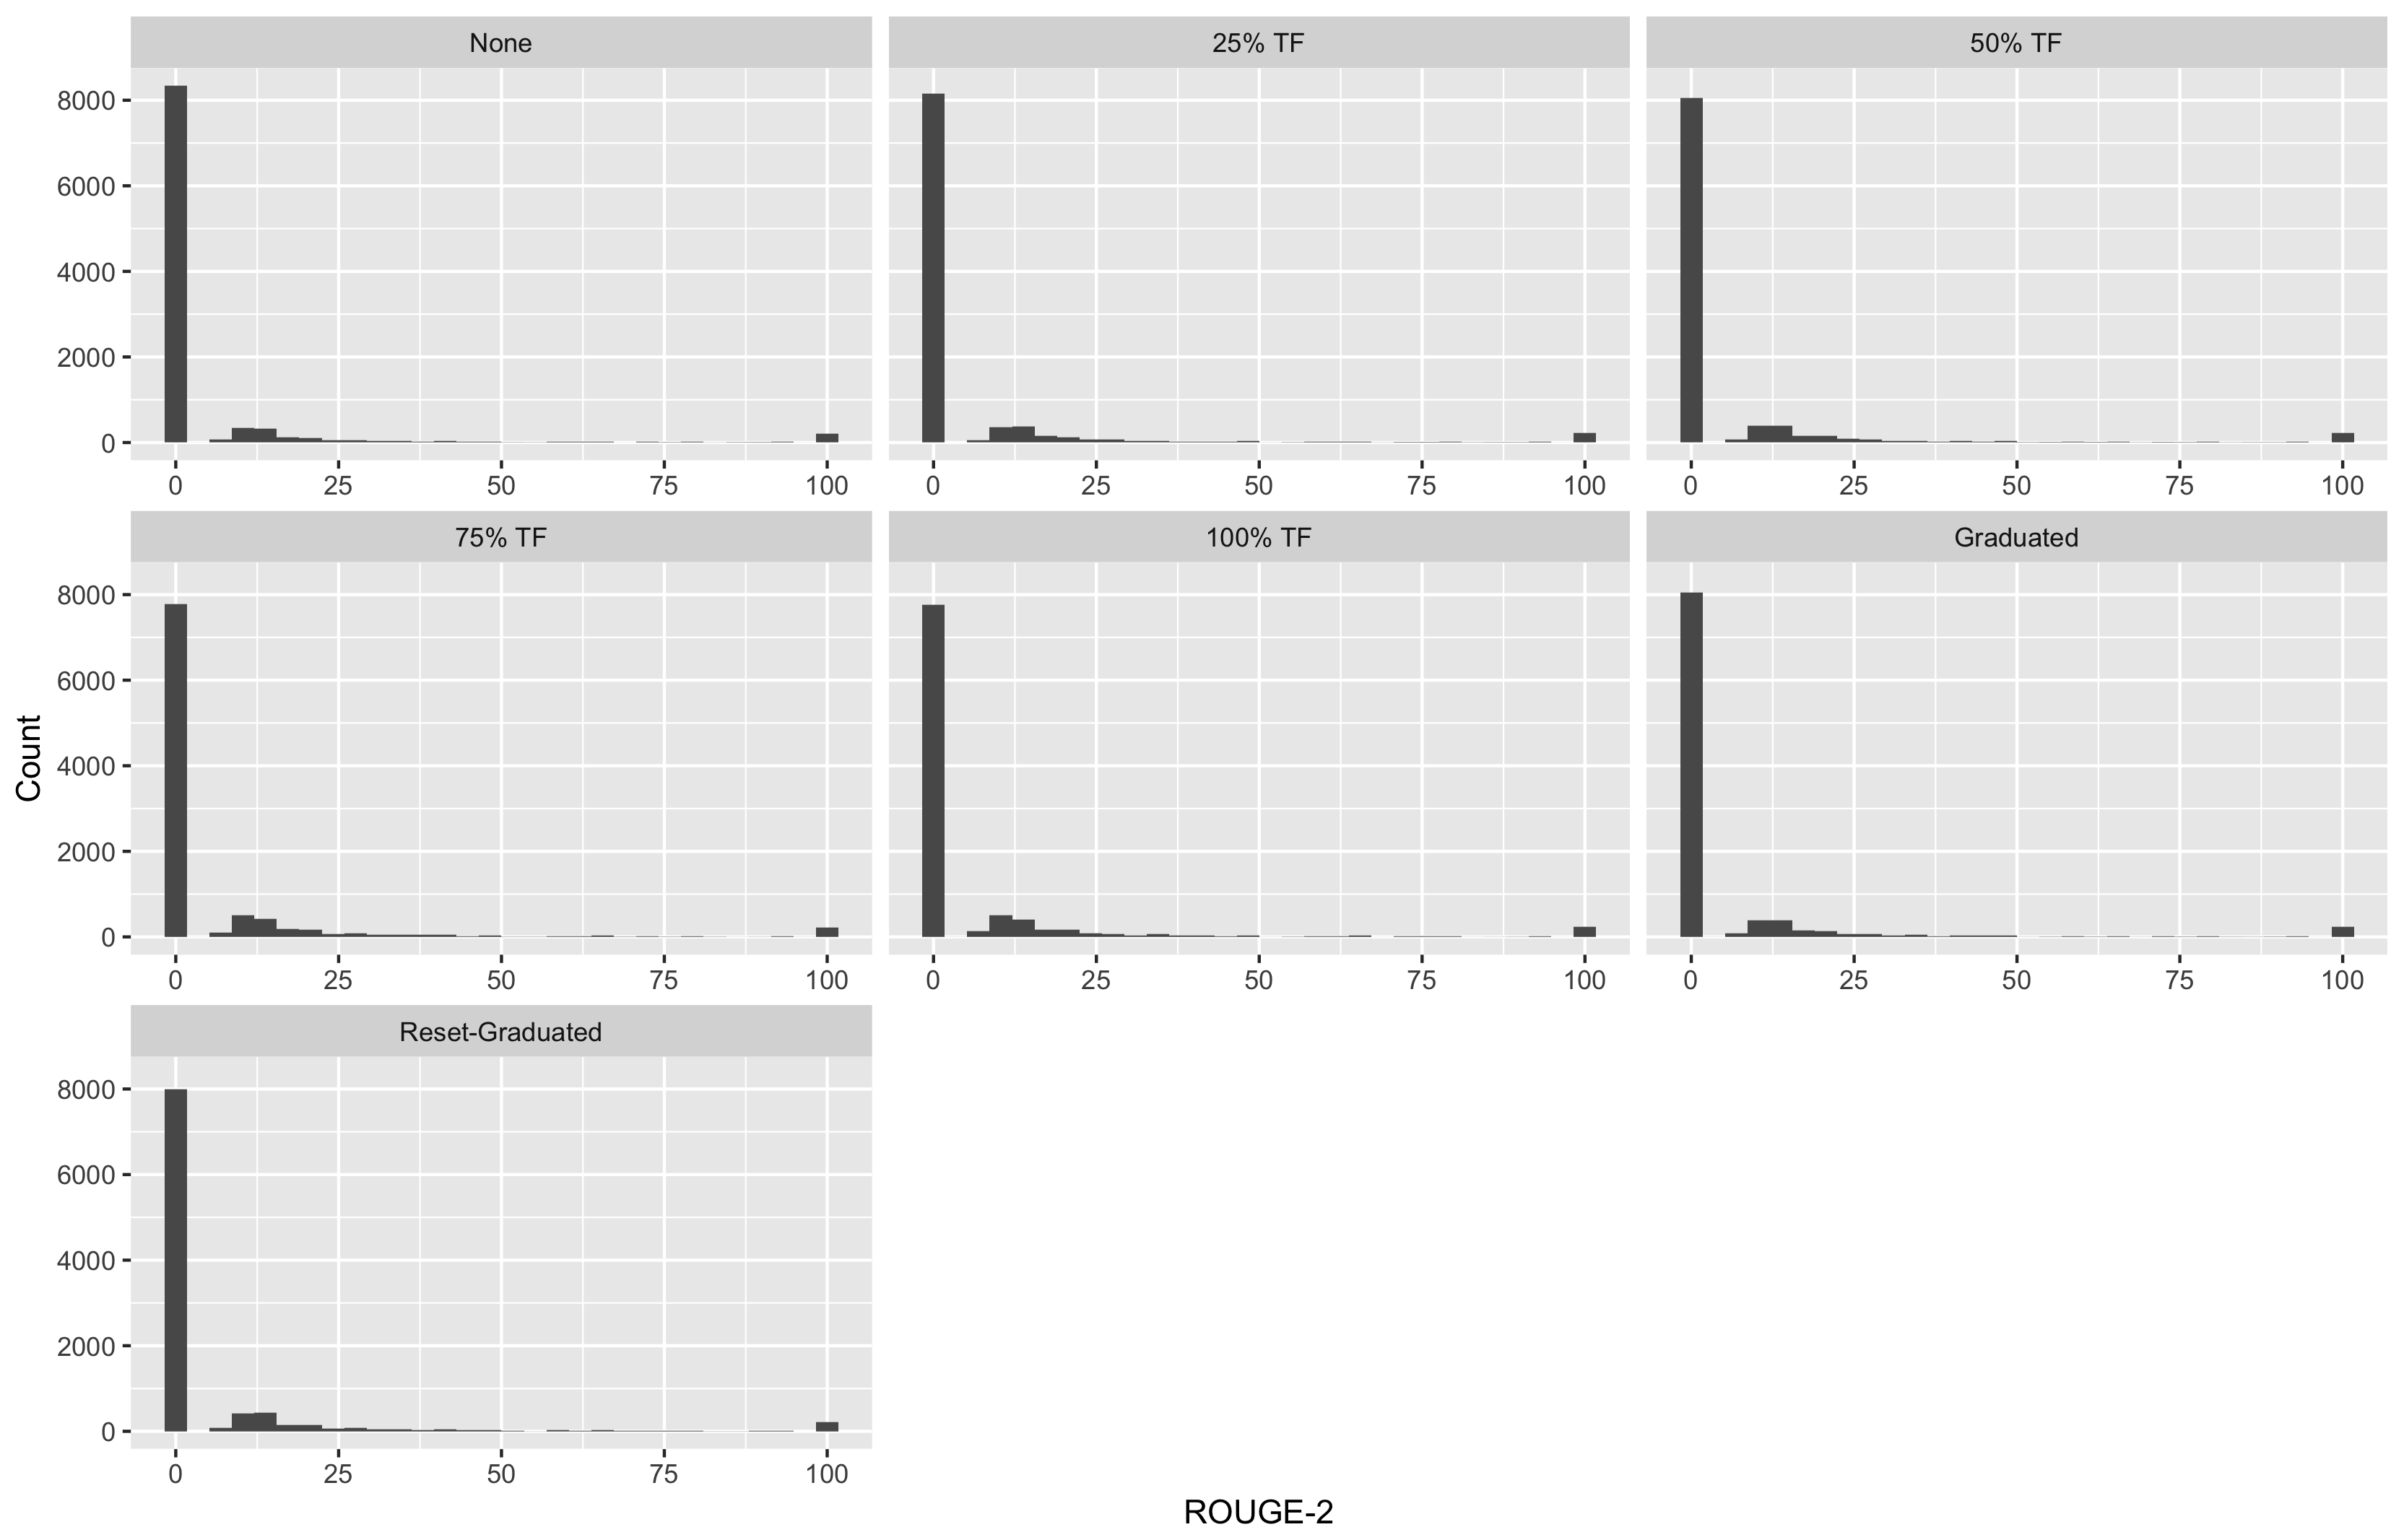
\includegraphics[width=0.8\textwidth]{../plots/test2/r2hists}
  \caption{Histograms of ROUGE-2 scores from all TF methods of Test 2}
  \label{fig:r2hists}
\end{figure}

Data non-normality can also be visualized via Q-Q Plots, as demonstrated for ROUGE-1 scores in Figure~\ref{fig:qqs}. A normal distribution would lie primarily near the regression line with dots randomly dispersed on either side~\cite{Ford2015}.

\begin{figure}[h]
  \centering
  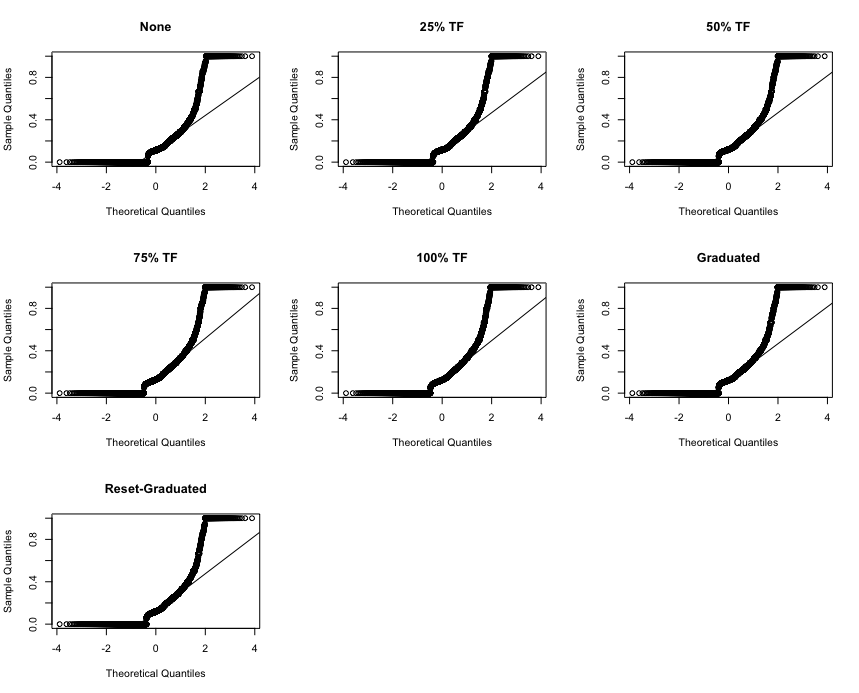
\includegraphics[width=0.8\textwidth]{../plots/test2/qqs}
  \caption{Q-Q Plots of ROUGE-1 scores for each TF Method of Test 2}
  \label{fig:qqs}
\end{figure}

Due to this skewedness, a Kruskal-Wallis test was used to compare the ROUGE results for each TF method across the three different tests. The results of the Kruskal-Wallis test can be viewed in Table~\ref{tab:kruskal}.

\begin{table}[h]
  \centering
  \begin{tabular}{| l | c | c |}
    \hline
    TF Method & ROUGE-1 & ROUGE-2\\
    \hline
    0\% & 0.481 & 0.262  \\
    25\% & 0.132 & 0.201  \\
    50\% & 0.162 & 0.307  \\
    75\% & 0.465 & 0.493  \\
    100\% & 0.632 & 0.577  \\
    Graduated & 0.175 & 0.770  \\
    Reset-Grad & 0.861 & 0.402  \\
    \hline
  \end{tabular}
  \caption{Kruskal-Wallis ROUGE-1 and ROUGE-2 p-values for various TF methods across three tests}
  \label{tab:kruskal}
\end{table}

Recall that values above 0.05 indicate a lack of statistical difference between the distributions of the data. Because all data fell within tolerance, we can safely assume no individual test benefitted from random chance. From here forward, analysis has only been conducted on the test 2. Having visualized the distribution of ROUGE scores and consolidated the analysis, we can now incorporate the appropriate metric for comparing TF methods: Wilcoxon averages and significance testing.

\subsubsection{Averages}\label{avg}
Tables~\ref{tab:avgROUGE1} and~\ref{tab:avgROUGE2} show the averages for ROUGE-1 and ROUGE-2, respectively. It bears repeating that, due to the necessary decrease in seq2seq architecture complexity, state-of-the-art results should not be expected. Rather, we are only hoping to compare various TF methods across the same datasets.

\begin{table}[h]
  \centering
  \begin{tabular}{| l | c | c |}
    \hline
    TF Method & Lower Bound & Upper Bound \\
    \hline
    0\% & 15.27  & 16.09 \\
    25\% & 16.04 & 16.86 \\
    50\% & 16.60 & 17.45 \\
    75\% & 17.76 & 18.59 \\
    100\% & 17.58 & 18.45 \\
    Graduated & 16.65 & 17.49 \\
    Reset-Grad & 16.52 & 17.36 \\
    \hline
  \end{tabular}
  \caption{ROUGE-1 bootstrapping averages for various TF methods}
  \label{tab:avgROUGE1}
\end{table}

\begin{table}[h]
  \centering
  \begin{tabular}{| l | c | c |}
    \hline
    TF Method & Lower Bound & Upper Bound \\
    \hline
    0\% & 4.997 & 5.688 \\
    25\% & 5.510 & 6.241 \\
    50\% & 5.692  & 6.403  \\
    75\% & 6.194  & 6.893  \\
    100\% & 6.223  & 6.964  \\
    Graduated & 5.692 & 6.421  \\
    Reset-Grad & 5.743 & 6.433  \\
    \hline
  \end{tabular}
  \caption{ROUGE-2 bootstrapping averages for various TF methods}
  \label{tab:avgROUGE2}
\end{table}

Perhaps surprisingly, these results appear to indicate that the highest levels of constantly held TF, 100\% and 75\%, resulted in the best possible ROUGE scores. This would appear to contradict the accepted wisdom that continual high levels of TF cause generative degradation. To validate these, though, we need to run paired Wilcoxon tests to test for significance.

\subsubsection{Paired Wilcoxon Tests}
We will run paired Wilcoxon tests on three different reference tests: all TF methods relative to no TF, all TF methods relative to 100\% TF, and graduated compared to reset-graduated. Recall from Section~\ref{stat} that the values reported are probabilities (p-values) that the differences in $\mu$ of the compared TF methods is 0. P-values $>$ 0.05 represent no statistically significant difference. We will first evaluate p-values with respect to no TF.

\begin{table}[h]
  \centering
  \begin{tabular}{| l | c | c |}
    \hline
    TF Method & ROUGE-1 & ROUGE-2 \\
    \hline
    25\% & 2.59E-3 & 9.77E-4  \\
    50\% & 2.46E-08 & 3.29E-07  \\
    75\% & 2.20E-16 & 2.20E-16  \\
    100\% & 2.20E-16 & 2.20E-16  \\
    Graduated & 1.43E-08 & 1.75E-7 \\
    Reset-Grad & 8.39E-08 & 6.57E-10  \\
    \hline
  \end{tabular}
  \caption{ROUGE paired Wilcoxon tests for various TF methods as compared to no teacher forcing}
  \label{tab:pairedNone}
\end{table}

It is immediately obvious that there are substantive differences between all TF methods relative to no TF, the least of which, unsurprisingly, being 25\% TF. Coupled with the fact that all TF methods had higher average confidence intervals, it is safe to assume that all TF methods under the parameters of the experiment score a higher ROUGE than not using TF. A simple ``greater-than'' Wilcoxon test confirms this to be true. Next we will evaluate all TF methods compared to 100\% TF, the industry standard at the moment.

\begin{table}[h]
  \centering
  \begin{tabular}{| l | c | c |}
    \hline
    TF Method & ROUGE-1 & ROUGE-2 \\
    \hline
    0\% & 2.20E-16 & 2.20E-16  \\
    25\% & 2.73E-10 & 1.15E-10  \\
    50\% & 1.81E-04 & 3.55E-06  \\
    75\% & 0.153 & 0.883  \\
    Graduated & 2.58E-04 & 5.78E-06  \\
    Reset-Grad & 8.14E-05 & 3.47E-4  \\
    \hline
  \end{tabular}
  \caption{ROUGE paired Wilcoxon tests for various TF methods as compared to 100\% teacher forcing}
  \label{tab:paired100}
\end{table}

Surprisingly, the differences in averages for 75\% and 100\% in Section~\ref{avg} seem to be substantiated by these paired Wilcoxon tests. We can see that 100\% teacher forcing is significantly different and of higher average confidence interval (See Sec.~\ref{avg}) than all TF methods besides 75\%. A ``greater-than'' Wilcoxon test confirms that these two TF methods have a statistically significantly higher mean than all other TF methods. Under the simplified conditions of this experiment, conventional wisdom is statistically incorrect. Because this project originally set out to research the effect of reset-graduated and graduated TF methods, we will analyze the statistical differences next, displayed in Figures~\ref{tab:pairedg}~and~\ref{tab:pairedrg}.

\begin{table}[h]
  \centering
  \begin{tabular}{| l | c | c | c | c |}
    \hline
    TF Method & ROUGE-1 & ROUGE-2 \\
    \hline
    0\% & 1.43E-08 & 1.75E-07  \\
    25\% & 7.79E-03 & 5.55E-2  \\
    50\% & 0.933 & 0.912  \\
    75\% & 3.72E-07 & 1.24E-05  \\
    100\% & 2.58E-04 & 5.78E-06  \\
    Reset-Grad & 0.778 & 0.343  \\
    \hline
  \end{tabular}
  \caption{ROUGE paired Wilcoxon tests for various TF methods as compared to graduated}
  \label{tab:pairedg}
\end{table}

\begin{table}[h]
  \centering
  \begin{tabular}{| l | c | c |}
    \hline
    TF Method & ROUGE-1 & ROUGE-2 \\
    \hline
    0\% & 8.38E-08  & 6.57E-10  \\
    25\% & 1.82E-2  & 4.23E-3  \\
    50\% & 0.842  & 0.292  \\
    75\% & 8.78E-08  & 6.31E-04  \\
    100\% & 8.14E-05  & 3.74E-04  \\
    Graduated & 0.778  & 0.343  \\
    \hline
  \end{tabular}
  \caption{ROUGE paired Wilcoxon tests for various TF methods as compared to reset-graduated}
  \label{tab:pairedrg}
\end{table}

As can be seen, graduated and reset-graduated TF methods have no statistically significant difference in generative performance. Perhaps unsurprisingly, both graduated and reset-graduated TF score similarly to 50\% constant TF, as these methods will, on average, have contributed TF approximately 50\% of the time. This is in contrast to the idea of presumed benefit from gradual tapering of TF, however.

Now that we have analyzed these various averages and their statistical differences, we will move on to loss over time.

\subsection{Loss over Time}\label{loss}
The original motivation behind TF was to speed up training. Consequently, we will evaluate the speed of convergence for all seven TF methods in all three tests conducted.

\begin{figure}[h]
  \centering
  Test 1 Losses\\
  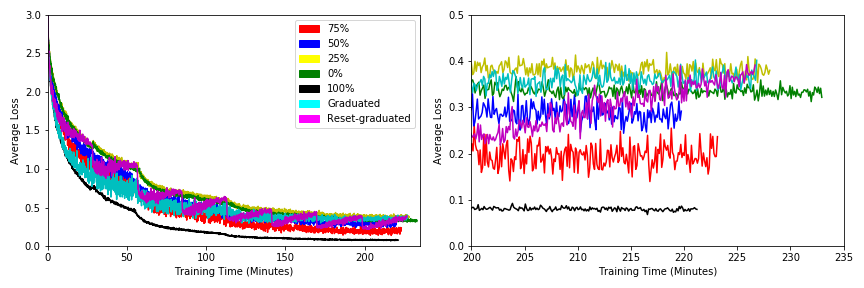
\includegraphics[width=0.8\textwidth]{../plots/test1comb}
  \caption{Average loss over time for every TF method for test 1}
  \label{fig:t1loss}
\end{figure}

\begin{figure}[h]
  \centering
  Test 2 Losses\\
  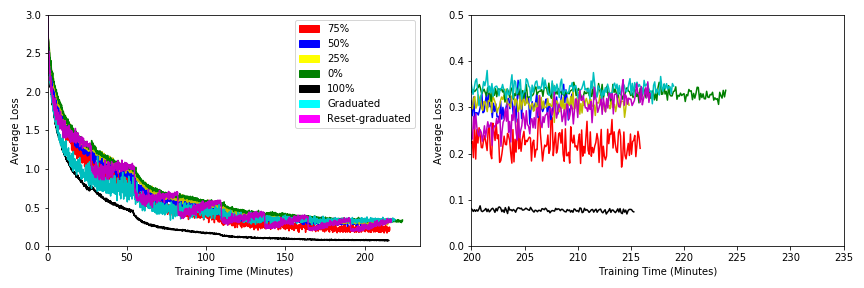
\includegraphics[width=0.8\textwidth]{../plots/test2comb}
  \caption{Average loss over time for every TF method for test 2}
  \label{fig:t2loss}
\end{figure}

\begin{figure}[h]
  \centering
  Test 3 Losses\\
  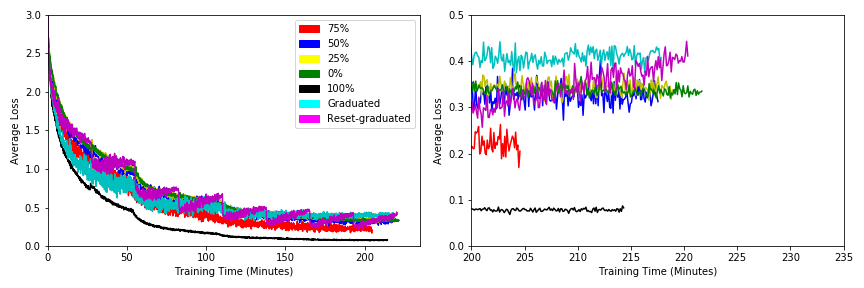
\includegraphics[width=0.8\textwidth]{../plots/test3comb}
  \caption{Average loss over time for every TF method for test 3}
  \label{fig:t3loss}
\end{figure}

There is a definite pattern amongst these three plots. 100\% TF converges noticably faster than all other TF tests. Additionally, 100\% TF had the lowest loss, unsurprising given the ROUGE findings. 75\% TF is consistently the second lowest for coverged loss. The rest all fall within the same general vacinity of one another. One interesting observation is how the Kruskal-Wallis scores showed no statistical difference between any of the ROUGE tests, yet many of the models from these techniques fluctuate by as much as 0.05. This would indicate that ROUGE outcomes are not particularly susceptible to such fluctuations at this loss level.

A second interesting observation is that converged loss proximity does not align with statistically significant over-performance on the ROUGE metric. According to the analysis on test 2 in Section~\ref{avg}, graduated, reset-graduated, 50\% and even 25\% all statistically outperformed 0\% TF, yet all final loss values are roughly the same. Indeed,  pulling the last recorded average loss for the functions results in the following losses:

\begin{itemize}
\item Graduated: 0.346
\item Reset-graduated: 0.329
\item 50\%: 0.327
\item 25\%: 0.305
\item 0\%: 0.337
\end{itemize}

This discrepancy between significant out-performance on ROUGE and comparative final loss values raises questions of whether ROUGE is a reliable metric, or whether the traditional cost function for these models needs could be better suited to specifically maximize ROUGE scores. However, given the lack of sophistication involved in ROUGE, I'm willing to bet the former. These observations raise some interesting new questions for future research.
\section{Conclusion}
In the Information Age, headlines have a ever-increasing presence in our lives. They show up in mobile notifications, in search engines, and all of the world's most popular websites. Due to the influence these hyper-condensed summaries can have, it is important to try to take steps towards ameliorating some of the negative consequences of their ubiquity. That said, the NLP community still has a lot of work to do in order to get to a point where they can start to address some of these pressing issues computationally. In these beginning stages, though, there are some interesting questions to be answered, not least of which is the question of optimal training parameters. As seen through this research, picking the correct TF method can have a statistically significant impact on generative results, as well as training time and converged loss.

The results of this experimentation have shown statistically significant ROUGE result improvement from using 75\% -- 100\% teacher forcing over any other methods tested. With the flexibility that PyTorch provides, there are an infinite number of TF strategies, but it's only a matter of time until we find the best way to automate and optimize it. For now, it is still a manually set variable, and typically only at 100\% out of necessity due to the restrictive nature of today's most popular deep learning libraries. For the abstractive summarization researcher who measures their success via ROUGE, however, this does not appear to be a problem. As is the case with many research projects, more questions were likely created than solved, but this opens the door to future research opportunities.

Sequence-to-sequence modelling is becoming more and more sophisticated as techniques and computability improve. Still, even now, there are many open questions that need addressing and I hope that the findings of this research can be utilized within the community.
\newpage
\section{Considerations for Future Work}
I believe the groundwork laid by this research leads to some interesting new questions, all of which are cause for further investigation. Some future projects may include:

\begin{itemize}
\item Running the models with greater computational resources to processes full dataset, add more encoding and decoding layers, increase hidden size, etc. See how model sophistication impacts the results found here.
\item Try a different domain. Seq2seq models are used very frequently in Neural Machine Translation (NMT) as well. Running the various TF experiments on a new domain could uncover some interesting results.
\item Invent new TF techniques, such as graduated steps every $n$ epochs.
\item Try running lower TF percentages only when a model has converged as a previous arbitrary TF percentage.
\item Implement the TF rate into PyTorch's autograd to learn, at any given iteration, whether or not TF should be allowed. Essentially turn teacher forcing into one of the tunable parameters that the model learns in order to best assist itself in minizing the model's loss.
\item Development of a more appropriate metric to judge computational comprehension than ROUGE
\end{itemize}

\newpage

\bibliography{../Bibliography/library}
\bibliographystyle{ieeetr}

\newpage

\begin{appendices}
  \section{Data Extraction}\label{app:extraction}
\begin{lstlisting}
  import os, re, random, glob, pickle, collections, bcolz, numpy as np, keras, sklearn, math, operator, gc, multiprocess as mp
  from tqdm import tqdm
  from random import shuffle
  from lxml import etree
  from itertools import islice

  MAX_HDLN_LEN = 30
  NUM_ART_SENTS = 1
  MAX_ART_LEN = 50 * NUM_ART_SENTS

  pattern = re.compile(r'''
                      # Don't care about matching beginning of string
  (                   # Start of Conditional (...|...)
                      ## First conditional
  (\(\s)*             # It could start with 1 or 0 '(' followed by possible whitespace
  \(+                 # One or More opening parentheses
  \-?                 # Possible starting '-' (-[LR]RB-)
  [A-Z\.,\'\`:]+      # One or More Capital letters and various punctuations
  \-?                 # Possible ending '-' (-(Right|Left) Parenthesis-)
  \$?                 # Zero or 1 '$'
  \s                  # Must be followed by whitespace

  |                   ## Second Conditional
  \(\s\$\s            # ( $
  |                   ## Third Conditional
  \)                  # Also replace ')' with ''
  |                   ## Fourth Conditional
  \n
  |                   ## Fifth Conditional
  by\b\w+\b\w+$)      # by Author
  ''', re.VERBOSE)

  def process_data(sentence):
    sentence = pattern.sub('', sentence)
    sentence = re.sub(r'(\`\`)|(\'\')', '"', sentence)
    sentence = re.sub(r'-RRB-', ')', sentence)
    sentence = re.sub(r'-LRB-', '(', sentence)
    sentence = re.sub(r'\.\.\.', ' ellipsis ', sentence)
    sentence = re.sub("([\d\"().,;:/_?!—])", r' \1 ', sentence).replace('-', ' ')
    sentence = re.sub(r'ellipsis', '...', sentence)
    sentence = re.sub(r'  *', ' ', sentence)
    sentence = sentence.lower().split()
    return sentence

  def extract_headline(hdln):
    for headline in hdln.itertext():
        headline = process_data(headline)
        return headline

  def extract_art_txt(txt, n_sents):
    sentences = []
    for sentence in islice(txt.itertext(), n_sents * 2):
        if sentence is not '\n':
            sentence = process_data(sentence)
            sentences += sentence
    return sentences

  def write_tab_seperated(file, headlines, articles, articles_per_file):
    global included, total, overall_total
    tree = etree.parse(file)
    root = tree.getroot()
    
    tot_arts = len(root)
    overall_total += tot_arts
    print(tot_arts," articles in this file. Extracting 100 article / headline pairs")
    rand_indicies = list(range(0,len(root))); shuffle(rand_indicies)
    
    num_processed = 0
    for rand_idx in rand_indicies:
        child = root[rand_idx]
        hdln = child.find('HEADLINE')
        txt = child.find('TEXT')

        if hdln is not None and txt is not None:
            total += 1
            headline = extract_headline(hdln)
            article = extract_art_txt(txt, n_sents = NUM_ART_SENTS)
            if len(headline) > MAX_HDLN_LEN or len(article) > MAX_ART_LEN: continue

            headline = ' '.join(headline)
            article = ' '.join(article)
            del child; gc.collect()
            num_processed += 1; included += 1
            if num_processed == articles_per_file: break
            headlines.append(headline)
            articles.append(article)
    del tree; gc.collect()

  DATA_PATH = '/Volumes/Alex Hard Drive/anno_eng_gigaword_5/data/xml/*'
  all_files = glob.glob(DATA_PATH); shuffle(all_files)

  articles = []; headlines = []
  included = 0
  total = 0
  overall_total = 0

  with open('test.txt', 'w') as f:
    f.write('')

  for file in tqdm(all_files):
    print('Parsing file: %s' % file)
    write_tab_seperated(file, headlines, articles, articles_per_file=120)
    percent_procd = included/total
    print('Total articles processed: {0} of {2} ({1:.1f}%)'.format(included, percent_procd * 100, total))

  with open('articles.pkl', 'wb') as f:
    pickle.dump(articles, f)

  with open('headlines.pkl', 'wb') as f:
    pickle.dump(headlines, f)
\end{lstlisting}
\newpage
\section{Training Functions}\label{app:train}
\begin{lstlisting}
def train(inp, targ, encoder, decoder, enc_opt, dec_opt, crit, teacher_forcing_ratio):
    decoder_input, encoder_outputs, hidden = encode(inp, encoder)
    target_length = targ.size()[1]
    
    enc_opt.zero_grad(); dec_opt.zero_grad()
    loss = 0

    if random.random() < teacher_forcing_ratio:
        for di in range(target_length):
            decoder_output, hidden = decoder(decoder_input, hidden, encoder_outputs)
            loss += crit(decoder_output, targ[:, di])
            decoder_input = targ[:, di]
            
    else: # feed output for next input
        for di in range(target_length):
            decoder_output, hidden = decoder(decoder_input, hidden, encoder_outputs)
            loss += crit(decoder_output, targ[:, di])
            topv, topi = decoder_output.data.topk(1);
            decoder_input = Variable(topi.squeeze()).cuda()

    loss.backward()
    enc_opt.step(); dec_opt.step()
    return loss.data[0] / target_length

  def trainEpochs(encoder, decoder, n_epochs, start_time, times_list, avg_loss_list, epochs_list,\
                print_every=200, lr=0.01, plot_loss_every=20, teacher_forcing = 'graduated',):
    print('LEARNING RATE: %f' % (lr))
    print_loss = 0 # Reset every print_every
    plot_loss = 0
    
    enc_opt = optim.Adam(req_grad_params(encoder), lr=lr)
    dec_opt = optim.Adam(decoder.parameters(), lr=lr)
    crit = nn.NLLLoss().cuda()
    
    for epoch in range(n_epochs):
        fra, eng = get_batch(fr_train, en_train, 128)
        inp = long_t(fra)
        targ = long_t(eng)
        
        try:
            isinstance(teacher_forcing, (str, float, int))
        except:
            raise TypeError
        
        if teacher_forcing == 'graduated':
            teacher_forcing_ratio = 1 - epoch/n_epochs
        elif teacher_forcing == 'full':
            teacher_forcing_ratio = 1
        elif teacher_forcing == 'none':
            teacher_forcing_ratio = 0
        elif teacher_forcing <= 1 and teacher_forcing >= 0:
            teacher_forcing_ratio = teacher_forcing
        else:
            raise ValueError
        
        loss = train(inp, targ, encoder, decoder, enc_opt, dec_opt, crit, teacher_forcing_ratio)
        print_loss += loss
        plot_loss += loss

        if epoch % print_every == 0 and epoch is not 0:
            print('%s\t%d\t%d%%\t%.4f' % (time_since(start_time, epoch / n_epochs), \
                                          epoch, epoch / n_epochs * 100, print_loss / print_every))
            print_loss = 0
        
        if epoch % plot_loss_every == 0 and epoch is not 0:
            times_list.append(calc_minutes(start_time))
            avg_loss_list.append(plot_loss / plot_loss_every)
            epochs_list.append(epoch)
            plot_loss = 0

  def multi_train(encoder, decoder, times_list, avg_loss_list, epochs_list, teacher_forcing_type):
    start_time = time.time()
    trainEpochs(encoder, decoder, 5000, start_time, times_list, avg_loss_list, epochs_list, lr=0.003, teacher_forcing=teacher_forcing_type)
    trainEpochs(encoder, decoder, 5000, start_time, times_list, avg_loss_list, epochs_list, lr=0.003, teacher_forcing=teacher_forcing_type)
    trainEpochs(encoder, decoder, 5000, start_time, times_list, avg_loss_list, epochs_list, lr=0.001, teacher_forcing=teacher_forcing_type)
    trainEpochs(encoder, decoder, 5000, start_time, times_list, avg_loss_list, epochs_list, lr=0.001, teacher_forcing=teacher_forcing_type)
    trainEpochs(encoder, decoder, 5000, start_time, times_list, avg_loss_list, epochs_list, lr=0.0003, teacher_forcing=teacher_forcing_type)
    trainEpochs(encoder, decoder, 5000, start_time, times_list, avg_loss_list, epochs_list, lr=0.0003, teacher_forcing=teacher_forcing_type)
    trainEpochs(encoder, decoder, 5000, start_time, times_list, avg_loss_list, epochs_list, lr=0.0001, teacher_forcing=teacher_forcing_type)
    trainEpochs(encoder, decoder, 5000, start_time, times_list, avg_loss_list, epochs_list, lr=0.00003, teacher_forcing=teacher_forcing_type)

  def fullgraduated_trainEpochs(encoder, decoder, total_epochs, start_time, times_list, avg_loss_list, epochs_list,\
                              print_every=200, lr=0.003, plot_loss_every=20):
    print("LEARNING RATE: %f" % (lr))
    print_loss = 0 # Reset every print_every
    plot_loss = 0
    
    enc_opt = optim.Adam(req_grad_params(encoder), lr=lr)
    dec_opt = optim.Adam(decoder.parameters(), lr=lr)
    crit = nn.NLLLoss().cuda()
    
    for epoch in range(total_epochs):
        fra, eng = get_batch(fr_train, en_train, 128)
        inp = long_t(fra)
        targ = long_t(eng)
        
        teacher_forcing_ratio = 1 - epoch/total_epochs
        
        loss = train(inp, targ, encoder, decoder, enc_opt, dec_opt, crit, teacher_forcing_ratio)
        print_loss += loss
        plot_loss += loss

        if epoch % print_every == 0 and epoch is not 0:
            print('%s\t%d\t%d%%\t%.4f' % (time_since(start_time, epoch / total_epochs), \
                                          epoch, epoch / total_epochs * 100, print_loss / print_every))
            print_loss = 0
        
        if epoch % plot_loss_every == 0 and epoch is not 0:
            times_list.append(calc_minutes(start_time))
            avg_loss_list.append(plot_loss / plot_loss_every)
            epochs_list.append(epoch)
            plot_loss = 0
        
        if epoch == 10000:
            lr = .001
            print("LEARNING RATE: %f" % (lr))
            enc_opt = optim.Adam(req_grad_params(encoder), lr=lr)
            dec_opt = optim.Adam(decoder.parameters(), lr=lr)
        elif epoch == 20000:
            lr = .0003
            print("LEARNING RATE: %f" % (lr))
            enc_opt = optim.Adam(req_grad_params(encoder), lr=lr)
            dec_opt = optim.Adam(decoder.parameters(), lr=lr)
        elif epoch == 30000:
            lr = .0001
            print("LEARNING RATE: %f" % (lr))
            enc_opt = optim.Adam(req_grad_params(encoder), lr=lr)
            dec_opt = optim.Adam(decoder.parameters(), lr=lr)
        elif epoch == 35000:
            lr = .00003
            print("LEARNING RATE: %f" % (lr))
            enc_opt = optim.Adam(req_grad_params(encoder), lr=lr)
            dec_opt = optim.Adam(decoder.parameters(), lr=lr)
\end{lstlisting}
\newpage
\section{Testing}
\begin{lstlisting}
  def evaluate(inp):
    decoder_input, encoder_outputs, hidden = encode(inp, encoder)
    target_length = maxlen

    decoded_words = []
    for di in range(target_length):
        decoder_output, hidden = decoder(decoder_input, hidden, encoder_outputs)
        topv, topi = decoder_output.data.topk(1)
        ni = topi[0][0];
        if ni==PAD: break
        decoded_words.append(en_vocab[ni])
        decoder_input = long_t([ni])
    
    return decoded_words

  def test(f_description):
    parent_dir = './Dissertation/rouge_eval/'+f_description
    ref_dir = parent_dir+'/reference/'
    system_dir = parent_dir+'/system/'
    
    if not os.path.exists(ref_dir): os.makedirs(os.path.dirname(ref_dir), exist_ok=True)
    if not os.path.exists(system_dir): os.makedirs(os.path.dirname(system_dir), exist_ok=True)
    
    for idx in range(len(fr_test)):
        real_sent = [en_id2w[t] for t in en_test[idx] if t != 0]
        if real_sent:
            with open(ref_dir + 'news%d_reference%d' % (idx, idx), 'w') as f:
                f.write(' '.join(real_sent))
        else:
            continue

        ids = long_t(fr_test[idx]); ids = ids.unsqueeze(0)
        translation = evaluate(ids)
        with open(system_dir + 'news%d_system%d' % (idx, idx), 'w') as f:
            f.write(' '.join(translation))
\end{lstlisting}
\end{appendices}

\end{document}
